\documentclass[12pt, a4paper, twoside]{article}

\usepackage[dutch]{babel}
\usepackage{hvaTemplate}
% \usepackage[hidelinks]{hyperref}
\usepackage[nameinlink,noabbrev,dutch]{cleveref}
\usepackage{csquotes}
\usepackage[backend=biber, style=ieee]{biblatex}
\usepackage{pgfplots}
\usepackage{siunitx}
\usepackage{caption}
\usepackage{subcaption}
\usepackage{graphicx}
\usepackage{xspace}
\usepackage{makecell}
\usepackage[perpage]{footmisc}
\sisetup{detect-all}


\pgfplotsset{compat=1.18}

\DeclareMathOperator\erfc{erfc}
\DeclareMathOperator\inverfc{inverfc}
\newcommand\SNR{\mbox{\textit{SNR}} }
\newcommand{\mcu}{nRF52810\xspace}
\newcommand\ph{\mathrm{pH}}


\DeclareSIUnit{\belmilliwatt}{Bm}

\addbibresource{references.bib}

% \setAuthor{\\Tycho Jöbsis (500845792)\\ Jochem Leijenhorst (500855372)\\ Illya Ustenko (500845492)}
\setAuthor{
    \\Groep 7
    \begin{table}[h!]
        \centering
        \begin{tabular}{ll}
            Jochem Leijenhorst  & (500855372)\\ 
            Tycho Jöbsis        & (500845792)\\ 
            Illya Ustenko       & (500845492)        
        \end{tabular}
    \end{table}
}
\extraInfo{Sensor modules}
\setTitle{Ontwerptraject pH sensor}

\graphicspath{ {img/} }

\numberwithin{equation}{section}

\DeclareSIUnit{\pH}{pH}

\makeatletter
\providecommand\add@text{}
\newcommand\tagaddtext[1]{%
\gdef\add@text{#1\gdef\add@text{}}}% 
\renewcommand\tagform@[1]{%
  \maketag@@@{\llap{\add@text\quad}(\ignorespaces#1\unskip\@@italiccorr)}%
}
\makeatother
  
\begin{document}
    \makeTitlepage

    %TODO: Hier komt een samenvatting in het Nederlands en Engels!

    \authorsCopyright
    \onecolumn
    \tableofcontents

    \newpage

    \section{Inleiding}

Voor het doen van onderzoek naar productiemethoden van drinkwater, het is belangrijk om tijdens verscheidene productie stappen de pH waarde van het water te kunnen meten. Om dat mogelijk te maken zal er in dit project gewerkt worden aan een eerste prototype van een pH sensormodule. Deze sensormodule zal rondom een ion gevoelige veld effect transistor (ISFET) worden ontwikkeld. De reden dat er geen gebruik gemaakt wordt van een glazen electrode pH sensoren is omdat deze duurder zijn om te produceren \cite{duroux1991ionpHISFETltspHmonitoring}. 

In het onderzoek waar deze sensormodule voor wordt ontwikkeld, zullen er meerdere van deze modules voor langere tijd data verzamelen. Om het makkelijk te maken om de pH meetdata te verzamelen heeft de sensormodule een draadloze verbinding nodig. Via deze draadloze verbinding is het dan mogelijk om de meetdata naar een basisstation te sturen. Dit basisstation is al ontwikkeld. 

Verder zal er gekeken worden naar methodes van energie harvesting om de levensduur van de sensormodule te verlengen. 

    \newpage

    \section{Theoretisch kader}
Voordat er ontworpen kan worden zal er eerst onderzoek gedaan moeten worden naar de werking van een ISFET. Dit is nodig om te weten hoe de pH uitgelezen kan worden.
Hiernaast zal er, omdat de module zichzelf ook moet kunnen opladen, ook onderzoek gedaan moeten worden naar energy harvesting.
Dit hoofdstuk zal ingaan op de bevindingen van het onderzoeken van beide onderwerpen.

\subsection{De werking van de ISFET}\label{sec:werkingISFET}
Een ISFET (Ion-Sensitive Field-Effect Transistor) is een FET die gevoelig is voor ionen \cite{modeling,isfetAsAnElectronicDevice,bergveld1985impactOfMosfetBasedSensors,bergveld2003thirtyYearsISFET}. Hierdoor is het mogelijk om met een ISFET pH-waardes te meten \cite{modeling,isfetAsAnElectronicDevice,bergveld1985impactOfMosfetBasedSensors,bergveld2003thirtyYearsISFET}. Een ISFET is in principe een MOSFET zonder gate. De ISFET gedraagt zich als een \si{\pH} afhankelijke MOSFET \cite{isfetAsAnElectronicDevice,bergveld1985impactOfMosfetBasedSensors,bergveld2003thirtyYearsISFET}.
% Er wordt een referentie-elektrode aan de te meten oplossing toegevoegd om de pH-waarde te kunnen meten. Deze referentie-elektrode kan gebruikt worden als de gate van de MOSFET \cite{van1987isfet,isfetAsAnElectronicDevice}. De drempelspanning van deze transistor is een functie van de pH-waarde van de gemeten oplossing. Een hogere pH-waarde geeft een lagere drempelspanning \cite{isfet,isfetAsAnElectronicDevice}.

\subsubsection{Werking van een MOSFET}
Om de werking van een ISFET te kunnen begrijpen moet er eerst worden gekeken naar hoe een MOSFET werkt.
MOSFETs kunnen in twee werkgebieden worden gebruikt: verzadigd en onverzadigd. Wanneer $U_{ds}<U_{gs}-U_{th}$ klopt bevindt een MOSFET zich in het onverzadigde gebied \cite{bergveld1985impactOfMosfetBasedSensors,inleidingInDeElektronicaWissenburgh}. Wanneer deze ongelijkheid niet klopt bevindt een MOSFET zich in het verzadigde gebied. \Cref{eq:IdMosfetUnsaturated} kan gebruikt worden om de drain stroom van een MOSFET in het onverzadigde gebied mee te berekenen. Wanneer een MOSFET zich echter in het verzadigde gebied bevindt kan \cref{eq:IdMosfetSaturated} gebruikt worden om de drainstroom van de MOSFET te berekenen \cite{elbasfun,inleidingInDeElektronicaWissenburgh,bergveld1985impactOfMosfetBasedSensors,isfetAsAnElectronicDevice,DonaldNeamenSemiconductorPhysicsAndDevicesBasicPrinciples}.
\begin{align}
    I_d{}&={}\mu C_{ox}\frac{W}{L}U_{ds}\left[\left(U_{gs}-U_{th}\right)-\frac{U_{ds}}{2}\right]
    \tagaddtext{[\si{\ampere}]} \label{eq:IdMosfetUnsaturated}\\
    %
    I_d{}&={}\mu C_{ox}\frac{1}{2}\frac{W}{L}\left(U_{gs}-U_{th}\right)^2
    \tagaddtext{[\si{\ampere}]} \label{eq:IdMosfetSaturated}
\end{align}
\begin{itemize}
    \item $I_d$ is de drain stroom van een MOSFET in [\si{\ampere}]
    \item $\mu$ is de ladingsdragers effectieve mobiliteit van een MOSFET in [\si{\volt^{-1}\,\second^{-1}}]
    \item $C_{ox}$ is de gate oxide capaciteit per opervlakte van een MOSFET in [\si{\farad\,\meter^{-2}}]
    \item $W$ is de breedte van een MOSFET in [\si{\meter}]
    \item $L$ is de lengte van een MOSFET in [\si{\meter}]
    \item $U_{ds}$ is de drain source spanning van een MOSFET in [\si{\volt}]
    \item $U_{gs}$ is de gate source spanning van een MOSFET in [\si{\volt}]
    \item $U_{th}$ is de drempelspanning\footnote{In het Engels heet de drempelspanning threshold voltage.} van een MOSFET in [\si{\volt}]
\end{itemize}

De gate van een MOSFET kan gezien worden als een condensator die op en ontladen moet worden \cite{DonaldNeamenSemiconductorPhysicsAndDevicesBasicPrinciples}. De waarde van een capaciteit kan met \cref{eq:calcCapacitance} worden berekend. In \cref{eq:calcCapacitance} is $\epsilon_0$ is de permitiviteit in vacuüm, $\epsilon_r$ is de relatieve permitiviteit en is afhankelijk van het materiaal tussen de twee platen van de condensator, $A$ het oppervlakte van de condensator en is $d$ de afstand tussen de twee condensator platen. \Cref{eq:calcCox} om $C_{ox}$ mee te berekenen is in essentie een gedifferentieerde versie van \cref{eq:calcCapacitance} over het oppervlakte van de condensator waarbij $t_{ox}$ de dikte van de gate oxide laag is \cite{DonaldNeamenSemiconductorPhysicsAndDevicesBasicPrinciples}.
\begin{equation} \label{eq:calcCapacitance}
    C=\frac{\epsilon_0\epsilon_rA}{d}
    \tagaddtext{[\si{\farad}]}
\end{equation}
\begin{equation}\label{eq:calcCox}
    C_{ox}=\frac{\epsilon_0\epsilon_r}{t_{ox}}
    \tagaddtext{[\si{\farad\,\meter^{-2}}]}
\end{equation}

De drempelspanning van een MOSFET is erg belangrijk om rekening mee te houden tijdens het ontwerpen van schakelingen die gebaseerd zijn rondom een MOSFET \cite{inleidingInDeElektronicaWissenburgh,DonaldNeamenSemiconductorPhysicsAndDevicesBasicPrinciples,verhoeven2007structured}. \Cref{eq:mosfetUth} laat zien hoe de drempelspanning van een MOSFET berekend kan worden. Hierbij is $Q_B$ de bulk depletion lading per oppervlakte en is $\phi_f$ het Fermi potentiaal verschil tussen het gedoteerde bulk silicium en het intrinsieke silicium \cite{bergveld1985impactOfMosfetBasedSensors}. Daarnaast is $U_{FB}$ de flatband spanning die wordt gegeven door \cref{eq:mosfetFB} \cite{bergveld1985impactOfMosfetBasedSensors,isfetAsAnElectronicDevice,DonaldNeamenSemiconductorPhysicsAndDevicesBasicPrinciples,bergveld2003thirtyYearsISFET}.
\begin{equation} \label{eq:mosfetUth}
    U_{th}=U_{FB}-\frac{Q_B}{C_{ox}}+2\phi_f
    \tagaddtext{[\si{\volt}]}
\end{equation}
\begin{equation} \label{eq:mosfetFB}
    U_{FB}=\frac{\Phi_M}{q}-\frac{\Phi_{si}}{q}-\frac{Q_{it}+Q_f}{C_{ox}}
    \tagaddtext{[\si{\volt}]}
\end{equation}
In \Cref{eq:mosfetFB} is $q$ de lading van het electron, zijn $Q_{it}$ en $Q_f$ de lading van de interface traps en de gefixeerde oxide lading. Beide zijn per oppervlakte \cite{bergveld1985impactOfMosfetBasedSensors}. Daarnaast is $\Phi_M$ metaal werkfunctie en is $\Phi_{si}$ de silicium werkfunctie \cite{bergveld1985impactOfMosfetBasedSensors,bergveld2003thirtyYearsISFET}.

\subsubsection{De drempelspanning van een ISFET}
Zoals in \cref{sec:werkingISFET} staat is de ISFET een MOSFET die gevoelig is voor \si{\pH} \cite{modeling,isfetAsAnElectronicDevice,bergveld1985impactOfMosfetBasedSensors,bergveld2003thirtyYearsISFET}. Het grootste verschil tussen een `normale' MOSFET en een ISFET, is dat de ISFET een MOSFET is met een losse gate. Zowel de gate (als elektrode) als de ISFET moeten in de zelfde vloeistof zijn om een \si{\pH} waarde te meten \cite{modeling,isfetAsAnElectronicDevice,bergveld1985impactOfMosfetBasedSensors,bergveld2003thirtyYearsISFET}.

De parameter van de ISFET die gevoelig is voor \si{\pH} is de drempelspanning \cite{isfetAsAnElectronicDevice,bergveld2003thirtyYearsISFET,bergveld1985impactOfMosfetBasedSensors}. De drempelspanning bestaat uit drie onderdelen zoals te zien is in \cref{eq:mosfetUth}. Hierbij is de flatband spanning afhankelijk van \si{\pH} \cite{isfetAsAnElectronicDevice,bergveld1985impactOfMosfetBasedSensors,bergveld2003thirtyYearsISFET}. Met \cref{eq:isfetUfb} kan voor een bepaalde \si{\pH} de flatband spanning worden berekend. In \cref{eq:isfetUfb} is $\chi^{sol}$ het oppervlakte dipole moment van de oplossing, $E_{ref}$ is het potentiaal van de referentie elektrode relatief aan het potentiaal van vacuüm. De term $E_{ref}$ bevat ook de metaalwerk functie $\Phi_M/q$ \cite{isfetAsAnElectronicDevice,bergveld2003thirtyYearsISFET,bergveld1985impactOfMosfetBasedSensors}. $\psi_0$ is een \si{\pH} afhankelijke variable \cite{isfetAsAnElectronicDevice,bergveld1985impactOfMosfetBasedSensors,bergveld2003thirtyYearsISFET}.
\begin{equation}\label{eq:isfetUfb}
    U_{FB}\left(\ph\right)=E_{ref}-\psi_0\left(\ph\right)+\chi^{sol}-\frac{\Phi_{si}}{q}-\frac{Q_{it}+Q_f}{C_{ox}}
    \tagaddtext{[\si{\volt}]}
\end{equation}

$\psi_0$ kan met \cref{eq:psi0} worden berekend. Hierbij is $k$ de constante van boltzmann, $T$ de temperatuur in kelvin, $\beta$ de chemische gevoeligheid van de oxide buiten laag, $\si{\pH}_{pzc}$ is de \si{\pH} van nul lading en \si{\pH} is de \si{\pH} van de oplossing \cite{bergveld2003thirtyYearsISFET,bergveld1985impactOfMosfetBasedSensors}.
\begin{equation}\label{eq:psi0}
    \psi_0\left(\ph\right)=2.303\frac{kT}{q}\left(\frac{\beta}{1+\beta}\right)\left(\ph_{pzc}-\ph\right)
    \tagaddtext{[\si{\volt}]}
\end{equation}
$\beta$ is afhankelijk van het type materiaal dat wordt gebruikt inplaats van de gate \cite{bergveld2003thirtyYearsISFET,bergveld1985impactOfMosfetBasedSensors}. Het is gebleken dat ISFET's die gebruik maken van $\mathrm{Al_{2}O_3}$ en $\mathrm{Ta_2O_5}$ een hogere $\beta$ hebben en daarmee dan ook gevoeliger voor veranderingen in \si{\pH} \cite{bergveld2003thirtyYearsISFET,bergveld1985impactOfMosfetBasedSensors}.

% \begin{equation}\label{eq:pHbeta}
%     \beta=2\frac{q}{kT}\frac{qN_s\sqrt{K_aK_b}}{C_{DL}}
% \end{equation}

\subsubsection{temperatuursafhankelijkheid van een ISFET}
De temperatuur gevoeligheidsanalyse valt buiten de scope van dit project. De geïntresseerde lezer wordt verwezen naar \cite{isfetAsAnElectronicDevice}. Uit \cite{isfetAsAnElectronicDevice} volgt dat een ISFET een temperatuursafwijking heeft van \qty{-1.39}{\milli\volt\,\kelvin^{-1}}.

% De ISFET is temperatuursafhankelijk \cite{isfet,isfetAsAnElectronicDevice}. Volgens de datasheet is de temperatuursafhankelijkheid gemiddeld $\qty{-0.2}{\milli\volt\per\kelvin}$\cite{Microsens-MSFET}. Om hiervoor te compenseren moet tijdens het meten ook de temperatuur gemeten worden. Ook zal bij het kalibreren de kalibratietemperatuur opgeslagen moeten worden. Wanneer er vervolgens gemeten wordt, zal de gemeten gate-source spanning door middel van het temperatuurverschil gecompenseerd moeten worden. Deze compensatie kan gedaan worden door middel van \cref{eq:tempComp}.

% \begin{equation}\label{eq:tempComp}
%     U_r = U_m + C_T(T_{meting} - T_{kalibratie})
%     \tagaddtext{[\si{\volt}]}
% \end{equation}
% Hierbij is $U_r$ de op temperatuur gecompenseerde ingangsspanning en $U_m$ de gemeten spanning.

% De richtingscoëfficiënt tussen de pH-waarde en de drempelspanning is constant, en varieert alleen van ISFET tot ISFET \cite{Microsens-MSFET}. Door deze als constant te nemen kan de pH-waarde berekend worden met een enkel kalibratiepunt.

% \begin{equation}\label{eq:calcPH}
%     \ph = C_{pH}(U_r - U_k) + \ph_k
%     \tagaddtext{[pH]}
% \end{equation}
% Hierbij is $a$ de richtingscoëfficiënt van de ISFET in pH/V, $U_r$ de op temperatuur gecompenseerde ingangsspanning, $\ph_k$ de pH waarde tijdens de kalibratie en $U_k$ de gemeten kalibratiespanning.

% \subsection{Empirisch onderzoek}
% \subsection{Gebruikersonderzoek}
% \subsection{Methodes}


\subsection{Energy Harvesting}
In veel toepassingen is het nuttig dat een sensormodule weinig onderhoud nodig heeft. Daarbij is het batterijleven van de sensormodule een van de belangrijkste aspecten. Energy harvesting is een manier om de levensuur van apparaten aanzienlijk te kunnen vergroten. Hierbij wordt energie uit de omgeving omgezet naar bruikbare elektrische energie. Er zijn meerdere methodes om energie te verkrijgen uit de omgeving. Voorbeelden van mogelijke energiebronnen zijn \cite{energyHarvesting}:
\begin{itemize}
    \item Kinetische energie
    \begin{itemize}
        \item Wind
        \item Water
        \item Vibratie
    \end{itemize}
    \item Elektromagnetische energie
    \begin{itemize}
        \item Zon
        \item Radio-frequentie
    \end{itemize}
    \item Thermische energie
    \item Atomische energie
    \begin{itemize}
        \item Radioactief verval
    \end{itemize}
\end{itemize}



    \newpage

    \section{Systeem specificaties}\label{sec:systemSpecifications}

% inleiden
Dit hoofdstuk zal ingaan op de systeem specificaties van de pH sensormodule. Hierbij zal ingegaan worden op wat de pH signalen zijn die worden verwacht, in welke omgeving de sensormodule moet werken en hoelang de tests kunnen duren.

% pH signaal
Voor dit onderzoek zijn pH schommelingen tot op \qty{0.05}{\pH} van interesse. Deze schommelingen kunnen optreden met een maximale frequentie van \qty{8}{\hertz}. Over het algemeen zal het water een pH waarde hebben tussen de pH 4 en de pH 8. Om er voor te zorgen dat er iets van marge in het pH meetbereik zit, zal de sensormodule een bereik van pH 2 tot pH 10 moeten kunnen meten. De onderzoekers hebben aangegeven dat het uitgangssignaal van de pH sensormodule een minimale signaal ruis verhouding (SNR) van \qty{36}{\decibel} moet hebben.

% basisstation
Het basisstation dat gebruikt zal worden bij het onderzoek is al ontwikkeld. Dit basisstation maakt gebruik van BLE voor de draadloze communicatie. De BLE implementatie van dit basisstation maakt gebruik van de \mcu voor de \qty{2.4}{\giga\hertz} BLE transceiver. 

% onderzoekslocatie/afstanden beschrijving
Voor dit onderzoek zullen de onderzoekers meerdere basins maken waarin chemische reacties plaatsvinden. Deze basins zullen voor het initiële onderzoek klein worden gehouden. Indien de resultaten van het onderzoek gunstig zijn is het mogelijk dat er op grotere schaal getest gaat worden. Tijdens dit initiële onderzoek zal de afstand tussen de pH sensormodules en het basisstation niet groter zijn dan \qty{10}{\meter}. Vanuit de onderzoekers is er gevraagd om er voor te zorgen dat de draadloze communicatie tussen de sensormodules en het basisstation 99.999\% betrouwbaar is. Hier volgt een bit error ratio (BER) eis van $1\times 10^{-5}$ uit.

% test periodes (tijd)
De onderzoekers hebben aangegeven dat de onderzoeken maximaal twee dagen (48 uur) duren. Het is van belang dat tijdens deze 48 uur de sensormodules niet uit het water hoeven te worden gehaald om opgeladen te worden. 


In \cref{tab:systemSpecs} zijn alle specificaties die hierboven zijn beschreven onder elkaar geplaatst.

\begin{table}[ht]
    \centering
    \begin{tabular}{|l|c c|l|}
        \hline
        Beschrijving                    & Min               & Max   & Eenheid           \\
        \hline 
        Afwijking                       &                   & 0.05  & pH                \\ 
        Bereik                          & 2                 & 10    & pH                \\
        Bandbreedte                     & 10                &       & Hz                \\
        $\mathrm{SNR}_{uit}$            & 36                &       & \qty{}{\decibel}  \\
        Rf afstand                      &                   & 10    & \qty{}{\meter}    \\
        Rf BER                          & $1\times10^{-5}$  &       & \%                \\
        Levensduur                      & 48                &       & \qty{}{\hour}     \\
        Gemiddeld gebruikte vermogen    &                   & 10    & mW                \\
        Energy harvesting               & $>$ 0             &       & mW                \\
        \hline
    \end{tabular}
    \caption{Systeemspecificaties.}
    \label{tab:systemSpecs}
\end{table}


% BER 0.01%

% Lijst met alle specificaties
% De pH sensormodule voor het onderzoek tot op \qty{0.05}{\pH} nauwkeurig de pH van water kunnen meten. Bij een aantal tests die gedaan zullen worden in dit onderzoek kan de pH met maximaal \qty{8}{\hertz} oscilleren. 

% Het bestaande basisstation maakt gebruik van Bluetooth Low Energy (BLE).  

% De pH sensor moet met grote nauwkeurigheid de pH waarde van een stof continu kunnen meten. 
% De enige beschikbare pH sensor die dit kan doen is een ISFET.
% Hierdoor zijn de specificaties deels gebaseerd op de specificaties van een ISFET pH sensor.

% De sensormodule heeft een eigen accu, en moet deze op kunnen laden zonder oplaadkabel.

% \begin{table}[ht]
    %     \centering
    %     \begin{tabular}{|l|r|}
        %         \hline
        %         BER             & 0.01\%  \\
        %         Energie per bit & J/b \\
        %         SNR             & \% \\
        %         Gevoeligheid Ontvanger & \% \\
        %         Zendvermogen    & dBm \\
        %         Ez              & \\ 
        %         Data rate       & b/s\\
        %         \hline
        %     \end{tabular}
        %     \caption{Specificaties draadloze verbinding.}
        %     \label{tab:wirelessSpec}
        % \end{table}

    \newpage

    \section{Ontwerp}\label{sec:ontwerp}
Het systeem bestaat uit 2 hoofdonderdelen: de sensormodule en een basisstation. De sensormodule meet de pH waarde van een oplossing, en verzend deze naar het basisstation. Het basisstation ontvangt de informatie en slaat deze informatie op.
In \cref{fig:functional} is dit te zien in een systeemdiagram.

\begin{figure}[!htbp]
    \centering
    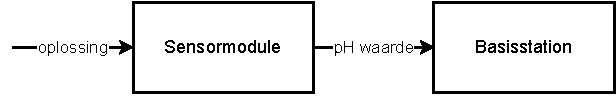
\includegraphics{toplevelDiagram}
    \caption[short]{Een diagram van het volledige systeem.}
    \label{fig:functional}
\end{figure}

Het sensormodule blok kan wederom opgedeeld worden in aparte blokken. Dit is te zien in \cref{fig:moduleDiagram}.

\begin{figure}[!htbp]
    \centering
    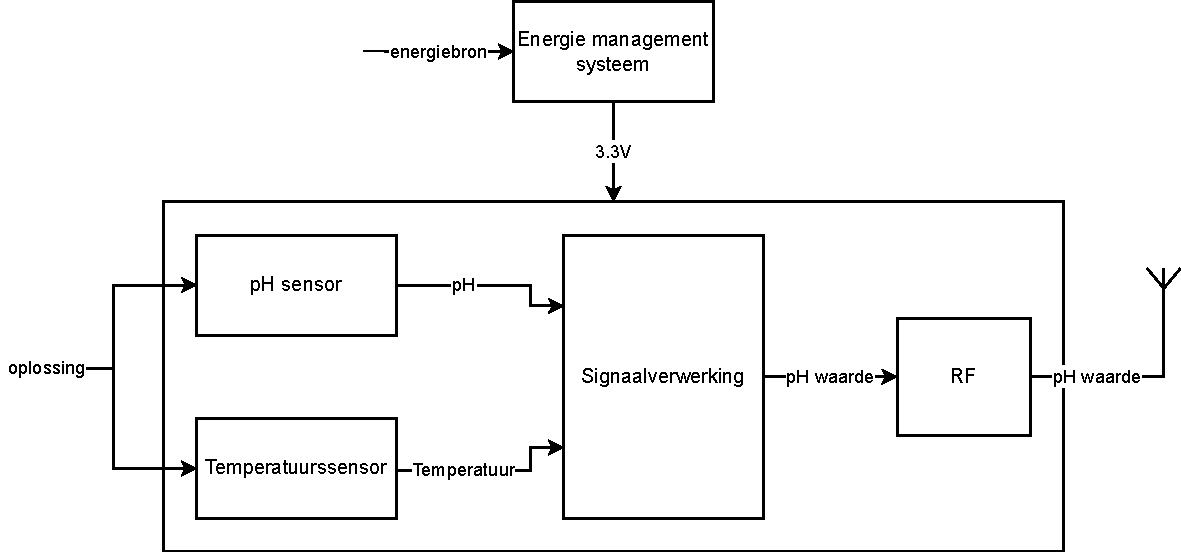
\includegraphics[width=0.75\textwidth]{moduleDiagram}
    \caption{Een systeemdiagram van de sensormodule.}
    \label{fig:moduleDiagram}
\end{figure}

\subsection{Functionele decompositie}
De sensormodule kan opgedeeld worden in 2 aparte systemen: de voeding, die verder wordt besproken in \cref{sec:voeding}, en de signaalverwerking.

De signaalverwerking bestaat zelf ook weer uit 2 onderdelen: het analoge gedeelte en het digitale gedeelte. In \cref{fig:analogeBewerkingsFunctie} is een decompositie te zien van de signaalbewerkingsfuncties die toegepast worden in het analoge gedeelte. In de komende paragrafen wordt elk van deze blokken apart besproken.

\begin{figure}[!htbp]
    \centering
    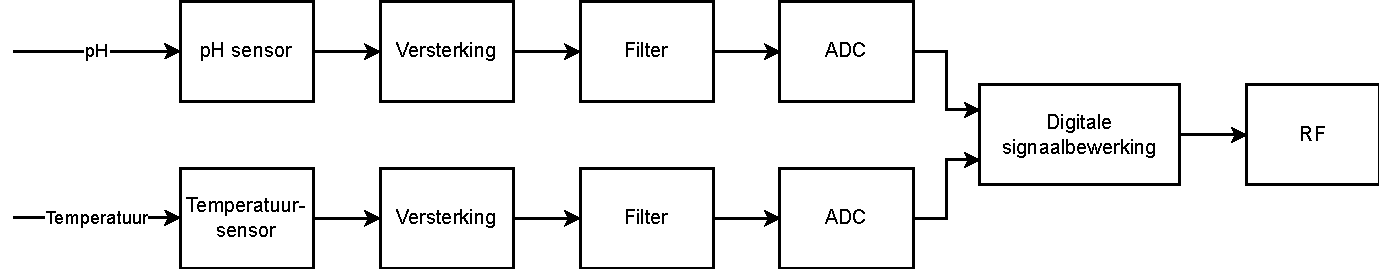
\includegraphics[width=0.95\textwidth]{analogeBewerkingsFunctie}
    \caption{Het analoge gedeelte van de signaalbewerking.}
    \label{fig:analogeBewerkingsFunctie}
\end{figure}


Het digitale gedeelte bestaat uit een aantal berekeningen. Deze berekeningen zijn nodig om de gemeten spanning om te rekenen naar een pH waarde. Hiervoor zijn een aantal kalibratiewaardes nodig, zoals besproken in \cref{sec:werkingISFET}. Het digitale gedeelte heeft als ingang een temperatuursafhankelijke spanning $U_T$ en een pH-afhankelijke spanning $U_{pH}$. Dit is te zien in \cref{fig:digitaleBewerkingsFunctie}. Beide van deze spanningen zijn de ruwe ADC waardes die gemeten worden, en hebben dus de hoogst mogelijke resolutie, namelijk de resolutie van de ADC. Voor beide van deze waardes zal de eenheid `bit' gebruikt worden.

Om op de uiteindelijk pH waarde te komen, wordt van de pH-afhankelijke spanning de pH-afhankelijke kalibratiespanning afgetrokken. Vervolgens wordt hier $\frac{pH_{kal}}{C_{pH}}$ bij opgeteld. Op deze manier kan er zo lang mogelijk met integers gewerkt worden die dezelfde resolutie hebben als de ingangs-ADC waarde. Het resultaat wordt vervolgens vermenigvuldigd met $C_{pH}$. Dit is de gevoeligheid van de sensor, in pH/bit.

Om de temperatuursafwijking te berekenen, wordt eerst van de temperatuursafhankelijke spanning $U_T$ de temperatuursafhankelijke kalibratiespanning $U_{T,kal}$ afgetrokken. Vervolgens wordt dit vermenigvuldigt met constante $C_T$. $C_T$ is de temperatuursafhankelijkheid van de pH-sensor, in pH/bit. Deze waarde kan afgeleid worden met de temperatuursafhankelijkheid van de pH-sensor die in de datasheet gegeven wordt in mV/K \cite{isfet}.

\begin{figure}[!htbp]
    \centering
    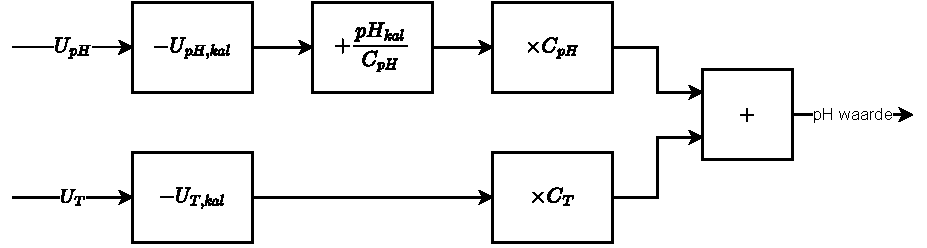
\includegraphics[width=0.95\textwidth]{digitaleBewerkingsFunctie}
    \caption{Het digitale gedeelte van de signaalbewerking.}
    \label{fig:digitaleBewerkingsFunctie}
\end{figure}


\subsection{De ISFET}

Aan de ingang van de signaalverwerking van de pH waarde, zit de sensor die deze pH waarde uitleest, zoals te zien in \cref{fig:pHInSchema}. Deze sensor meet de pH waarde van de te meten oplossing. De sensor die wordt gebruikt is een ISFET halfgeleider.
\begin{figure}[!htbp]
    \centering
    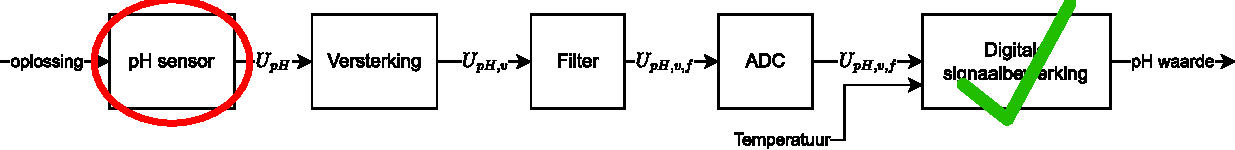
\includegraphics[width=0.95\textwidth]{signaalverwerking_pH.pdf}
    \caption{Het onderdeel van \cref{fig:analogeBewerkingsFunctie} waar dit hoofdstuk over gaat.}
    \label{fig:pHInSchema}
\end{figure}

De pH sensor heeft als ingang een oplossing met een pH waarde van pH 2 tot pH 10. De uitgang is een spanning tussen de \qty{1.8}{\volt} en \qty{2.2}{\volt} \cite{isfet}, die lineair afhankelijk is van de pH waarde. Dit is te zien in \cref{fig:uitleesBlok}.

\begin{figure}[!htbp]
    \centering
    \def\svgwidth{0.4\textwidth}
    \input{img/uitleesBlok.pdf_tex}
    \caption{De in- en uitgangen van de uitleesschakeling.}
    \label{fig:uitleesBlok}
\end{figure}


\subsubsection{De drempelspanning van de ISFET uitlezen} \label{sec:ISFETLees}
Wanneer de ISFET in aanraking komt met een oplossing, verandert de gate-source drempelspanning op basis van de pH waarde van deze oplossing \cite{bergveld2003thirtyYearsISFET,bergveld1985impactOfMosfetBasedSensors}. Om deze uit te lezen kan een regelsysteem gebruikt worden om de drain-source spanning en stroom van de ISFET mee in te stellen.

Er zijn meerdere mogelijke implementaties mogelijk voor dit regelsysteem. Twee hiervan zijn afgebeeld in \cref{fig:measureCircuits}.
Elk van deze schakelingen gebruikt een nullor om de drain-source spanning van de ISFET gelijk te houden. Ook gebruikt elk van deze schakelingen een referentiespanning. De implementatie van deze referentiespanning wordt verder besproken in \cref{sec:referenceVoltage}.

De drain-source spanning $U_{ds}$ en drain-source stroom $I_{ds}$ zijn van te voren gedefinieerd. Deze zijn te vinden in de datasheet van de ISFET \cite{isfet}. Uit deze twee waardes kunnen de referentiespanningen en weerstandswaardes van de schakelingen gevonden worden.
Voor de schakeling in \cref{fig:measureCurrent} is de spanningsreferentie te vinden door middel van \cref{eq:URefSource}.
\begin{equation}\label{eq:URefSource}
    U_{ref,s} = U_{dd} - U_{ds}
    \tagaddtext{[\si{\volt}]}
\end{equation}
Voor \cref{fig:measureResistor} is de referentiespanning gelijk aan de drain-source spanning, te zien in \cref{eq:URefDrain}.
\begin{equation}\label{eq:URefDrain}
    U_{ref,d} = U_{ds}
    \tagaddtext{[\si{\volt}]}
\end{equation}
Voor de waarde van de weerstand in \cref{fig:measureResistor} kan \cref{eq:measureResistorVal} gebruikt worden.
\begin{equation}\label{eq:measureResistorVal}
    R = \frac{U_{dd} - U_{ds}}{I_{ds}}
    \tagaddtext{[\si{\ohm}]}
\end{equation}


\begin{figure}[!htbp]
    \centering
    \begin{subfigure}[b]{0.45\textwidth}
        \centering
        \def\svgwidth{\textwidth}
        \input{img/ISFETCircuitBest.pdf_tex}
        \caption{Met een weerstand aan de drain.}
        \label{fig:measureResistor}
    \end{subfigure}
    \hfill
    \begin{subfigure}[b]{0.45\textwidth}
        \centering
        \def\svgwidth{\textwidth}
        \input{img/ISFETCircuit.pdf_tex}
        \caption{Met een stroombron aan de source.}
        \label{fig:measureCurrent}
    \end{subfigure}
    \caption{De uitleesschakelingen voor de ISFET.}
    \label{fig:measureCircuits}
\end{figure}

Beide schakelingen hebben voor- en nadelen.
Bij de schakeling in \cref{fig:measureResistor} zit de source van de ISFET direct verbonden met de ground. Dit heeft als voordeel dat de uitgang van de nullor gelijk is aan de gate-source spanning. Hierdoor hoeft de nullor lagere spanningen te genereren om de gate-source spanning van de ISFET naar de goede waarde te krijgen. De spanning die de nullor moet genereren in het geval van een drain weerstand is te vinden door middel van \cref{eq:nullorVoltageDrain}. In het geval van een stroombron aan de source is dat \cref{eq:nullorVoltageSource}.

\begin{equation}\label{eq:nullorVoltageDrain}
    U_{nullor,d} = U_{gs}
    \tagaddtext{[\si{\volt}]}
\end{equation}
\begin{equation}\label{eq:nullorVoltageSource}
    U_{nullor,s} = U_{gs} + U_{ref,s}
    \tagaddtext{[\si{\volt}]}
\end{equation}

De schakeling met een stroombron aan de source heeft de mogelijkheid om betere ruiseigenschappen te hebben. De stroombron kan ook een hogere impedantie hebben dan de weerstand. Het vermogensverbruik van de schakeling in \cref{fig:measureResistor} is echter duidelijk minder, dus is dit de schakeling die gebruikt zal worden.

\subsubsection{Ruis van de ISFET uitleesschakeling}

De meetschakeling heeft een aantal ruisbronnen. De nullor heeft een ingangsstroom- en spanningsruisbron. Daarnaast genereert de weerstand ook thermische ruis. Deze ruisbronnen zijn te zien in \cref{fig:measureNoise}.
\begin{figure}[!htbp]
    \centering
    \def\svgwidth{0.6\textwidth}
    \input{img/ISFETCircuitBestNoise.pdf_tex}
    \caption{De ruisbronnen van de meetschakeling.}
    \label{fig:measureNoise}
\end{figure}


Omdat $U_{ds}$ en $I_{ds}$ van de ISFET niet veranderen, kan de impedantie ervan gezien worden als weerstand, met een waarde van $\frac{U_{ds}}{I_{ds}}$. Hierdoor wordt er een nieuwe ruisbron $i_{n,ds}$ toegevoegd. Met deze weerstand kunnen de bronnen $i_{n,ref}$, $i_{n,R}$ en $i_{n,ds}$ worden getransformeerd naar een spanningsbron $u_{n,in}$ aan de ingang van de nullor.
Vervolgens kan deze, samen met de spanningsruisbronnen $u_{n,ref}$ en $u_{n,n}$ naar de uitgang getransformeerd worden. Dit komt uit op een enkele spanningsruisbron aan de uitgang, zoals te zien is in \cref{fig:measureNoiseMoved}. De spectrale spanningsruis dichtheid van deze ruisbron is te berekenen door middel van \cref{eq:measureNoiseOut}.

\begin{equation}\label{eq:measureNoiseOut}
    S_{u_{{n,out}}} = \left(S_{u_{{n,ref}}} + S_{u_{{n,n}}} + S_{i_{n,in}}\left(Z_{fet} // R\right)^2\right) \cdot H^2(\ph)
    \tagaddtext{[\si{\volt\squared\per\hertz}]}
\end{equation}
\begin{equation}
    S_{i_{{n,in}}} = S_{i_{{n,n}}} + S_{i_{{n,R}}} + S_{i_{{n,ds}}}
    \tagaddtext{[\si{\ampere\squared\per\hertz}]}
    \label{eq:measureNoiseCurrentIn}
\end{equation}


De definities van deze ruisbronnen zijn te vinden in \cref{tab:measureNoiseValues}.

\begin{table}[!htbp]
    \centering
    \begin{tabular}{c|l}
        Ruisbron & Waarde \\
        \hline
        $S_{u_{{n,ref}}}$ & Zie \cref{sec:referenceVoltage} \\
        $S_{u_{{n,n}}}$   & Implementatie nullor \\
        $S_{i_{{n,n}}}$   & Implementatie nullor \\
        $S_{i_{n,in}}$    & \Cref{eq:measureNoiseCurrentIn} \\
        $S_{i_{{n,R}}}$   & $\frac{4kT}{R}$ \\
        $S_{i_{{n,ds}}}$  & $4kT\frac{I_{ds}}{U_{ds}}$ \\
    \end{tabular}
    \caption{Waar de waardes van de ruisbronnen vandaan gehaald kunnen worden.}
    \label{tab:measureNoiseValues}
\end{table}

\begin{figure}[!htbp]
    \centering
    \def\svgwidth{0.6\textwidth}
    \input{img/ISFETCircuitBestNoiseMoved.pdf_tex}
    \caption{De meetschakeling met verschoven ruisbronnen.}
    \label{fig:measureNoiseMoved}
\end{figure}

De overdracht van deze schakeling is gelijk aan de uitgangsspanning gedeeld door de ingangsspanning van de nullor. Door de werking van de schakeling blijft de ingangsspanning altijd gelijk en is de uitgangsspanning lineair afhankelijk van de pH waarde. Hierdoor is de overdracht $H(\ph)$ een functie van de gemeten pH waarde.

Deze overdrachtsfunctie is gedefinieerd in \cref{eq:measureTransfer}, en is een functie van de uitgangsspanning. De uitgangsspanning is een functie van de pH waarde, en is te vinden in \cref{eq:measureOutVoltage}. Hierin is $C_{pH}$ de gevoeligheid van de sensor, die gegeven wordt in $\si{\milli\volt\per\ph}$, en is $U_7$ de uitgangsspanning op pH 7.

\begin{equation}
    H(\ph) = \frac{U_o(\ph)}{U_{ref}}
    \label{eq:measureTransfer}
\end{equation}

\begin{equation}\label{eq:measureOutVoltage}
    U_o(\ph) = C_{pH}\ph + U_7
    \tagaddtext{[\si{\volt}]}
\end{equation}
Door de hoogste uitgangsspanning $U_{o,max}$ te nemen, kan de maximale uitgangsruis berekend worden. Deze is te vinden in \cref{eq:measureNoiseFull}.

\begin{equation}\label{eq:measureNoiseFull}
    S_{u_{{n,out}}} = \left(S_{u_{{n,ref}}} + S_{u_{{n,n}}} + S_{i_{{n,in}}}\left(Z_{fet} // R\right)^2\right) \cdot \left(\frac{U_{o,max}}{U_{ref}}\right)^2
    \tagaddtext{[\si{\volt\squared\per\hertz}]}
\end{equation}

Aangezien er geen frequentieafhankelijkheden voorkomen kan de uitgangsspanningsruis uitgerekend worden door de spectrale ruisdichtheid te vermenigvuldigen met de bandbreedte. Dit wordt gedaan in \cref{eq:measureNoiseVoltage}.
\begin{equation}\label{eq:measureNoiseVoltage}
    u_{n,out} = \sqrt{B \cdot S_{u_{{n,out}}}}
    \tagaddtext{[\si{\volt}]}
\end{equation}

\subsubsection{Vermogen van de ISFET uitleesschakeling}
Het vermogensverbruik van deze schakeling is gedefinieerd in \cref{eq:measurePower}, waar $P_n$ het vermogensverbruik van de nullor implementatie is.
\begin{equation}\label{eq:measurePower}
    P = P_n + U_{dd}I_{ds}
\end{equation}


% \subsubsection{Versterker}
% Aangezien de uitgang van de ISFET een meetbare spanning produceert (\qty{1.8}{\volt} tot \qty{2.2}{\volt} volgens \cite{isfet}) zal er geen versterker nodig zijn om de pH waarde te kunnen meten. Wel zou een level-shifter gebruikt kunnen worden in combinatie met een versterker om zo het volledige bereik van de ADC te gebruiken. Dit voegt echter meer ruis en complexiteit toe aan het systeem, waardoor er in deze iteratie voor is gekozen om dit niet te doen.
%TODO: dit^^
\subsection{Spanningsreferentie}\label{sec:referenceVoltage}

De ISFET uitleesschakeling heeft een spanningsreferentie nodig om te werken.
% TODO: Vertel misschien over andere methoden.
Hiervoor is als implementatie een spanningsdeler gekozen. De schakeling van deze spanningsdeler is te zien in \cref{fig:divider}.
De condensator wordt gebruikt om ruis te verminderen op hogere frequenties, en dient ook als filter voor hoogfrequente storing in de voedingsspanning.

\begin{figure}[!htbp]
    \centering
    \def\svgwidth{0.5\textwidth}
    \subsection{Spanningsreferentie}\label{sec:referenceVoltage}

De ISFET uitleesschakeling heeft een spanningsreferentie nodig om te werken.
% TODO: Vertel misschien over andere methoden.
Hiervoor is als implementatie een spanningsdeler gekozen. De schakeling van deze spanningsdeler is te zien in \cref{fig:divider}.
De condensator wordt gebruikt om ruis te verminderen op hogere frequenties, en dient ook als filter voor hoogfrequente storing in de voedingsspanning.

\begin{figure}[!htbp]
    \centering
    \def\svgwidth{0.5\textwidth}
    \input{img/divider.pdf_tex}
    \caption{De schakeling van de spanningsdeler die dient als spanningsreferentie.}
    \label{fig:divider}
\end{figure}

De overdracht van deze spanningsdeler is te vinden in \cref{eq:dividerTransfer}.
\begin{equation}\label{eq:dividerTransfer}
    H(s) = \frac{U_{ref}(s)}{U_{dd}(s)} = \frac{R_2}{R_1 + R_2 + R_2Cs}
\end{equation}

\subsubsection{Vermogen}
Het vermogen dat de spanningsdeler dissipeert, kan met \cref{eq:dividerPower} berekend worden.
\begin{equation}\label{eq:dividerPower}
    P(s) = U_{dd}^2(s)\frac{1+R_2Cs}{R_1 + R_2 + R_1R_2Cs}
    \tagaddtext{[\si{\watt}]}
\end{equation}
Met een constante DC ingangsspanning kan dit vereenvoudigd worden naar \cref{eq:dividerPowerSimple}.
\begin{equation}\label{eq:dividerPowerSimple}
    P = \frac{U_{dd}^2}{R_1 + R_2}
    \tagaddtext{[\si{\watt}]}
\end{equation}

\subsubsection{Ruis}
Om de ruis van deze schakeling te berekenen moet een aantal stappen genomen worden. Aangezien de ingangsbron $U_{dd}$ een spanningsbron is, kan deze als kortsluiting genomen worden. Op deze manier kunnen de twee weerstanden parallel genomen worden, en verandert de schakeling in een simpel RC filter. In \cref{fig:dividerNoise} is deze omgebouwde schakeling te zien.

\begin{figure}[!htbp]
    \centering
    \def\svgwidth{0.35\textwidth}
    \input{img/dividerNoise.pdf_tex}
    \caption{De omgebouwde schakeling om ruis mee te berekenen.}
    \label{fig:dividerNoise}
\end{figure}

\noindent
Voor de spectrale spanningsruisdichtheid aan de uitgang $U_{ref}$ kan \cref{eq:dividerNoiseLaplace} worden opgesteld.
\begin{equation}\label{eq:dividerNoiseLaplace}
    S_{n,u_{ref}} = 4kTR_e\left(\frac{1}{1 + R_eCs}\right)^2
    \tagaddtext{[\si{\volt\squared\per\hertz}]}
\end{equation}
Wanneer de absolute waarde van de ruis wordt genomen, kan deze over de bandbreedte geïntegreerd worden. Dit resulteert in \cref{eq:dividerNoiseInt}, waar B de bandbreedte is.
\begin{equation}\label{eq:dividerNoiseInt}
    u_{n,ref}^2 = 4kTR_e\int_{B} \frac{1}{1 + (2\pi f R_e C)^2} df
    \tagaddtext{[\si{\volt\squared}]}
\end{equation}
Met een oneindige bandbreedte komt deze integraal uit op \cref{eq:dividerNoiseIntegratedInf}.
\begin{equation}\label{eq:dividerNoiseIntegratedInf}
    u_{n,ref}^2 = \lim_{f\rightarrow\infty}\frac{2kT}{\pi C} \arctan(2\pi f R_eC)
    \tagaddtext{[\si{\volt\squared}]}
\end{equation}
Aangezien de inverse tangens $\frac{\pi}{2}$ nadert, komt dit limiet uit op \cref{eq:dividerNoise}.
\begin{equation}\label{eq:dividerNoise}
    u_{n,ref}^2 = \frac{kT}{C}
    \tagaddtext{[\si{\volt\squared}]}
\end{equation}
Omdat een oneindige bandbreedte gebruikt is om op \cref{eq:dividerNoise} te komen, berekend deze de ruis in het ergste geval. De weerstandswaardes van $R_1$ en $R_2$ zijn hierbij irrelevant. Hierdoor is ruis geen bepalende factor meer tijdens het kiezen van de weerstandswaardes van de spanningsdeler, en kunnen deze volledig gebaseerd worden op vermogensverbruik. Volgens \cref{eq:dividerPowerSimple} is het vermogen omgekeerd evenredig met de som van de weerstandswaardes. Daarbij zit de uitgang van de spanningsdeler direct verbonden met de ingang van een nullor. Er hoeft dus geen rekening gehouden te worden met de uitgangsimpedantie van de spanningsbron. Hierdoor is het voor het vermogensverbruik voordelig om de weerstandswaardes zo hoog mogelijk te kiezen.

\subsubsection{Simulatie}

Om te verifiëren dat de spanningsreferentie goed werkt, is er een aantal simulaties uitgevoerd.

In \cref{fig:referenceSimFreq} is het resultaat van een AC simulatie te zien. Hier is $H(f)$ de overdracht van $U_{dd}$ naar

\begin{figure}[!htbp]
    \centering
    \pgfplotsset{width=0.7\textwidth}
    \input{plots/referenceSimFreq.tex}
    \caption{Het resultaat van een AC simulatie van de spanningsreferentie.}
    \label{fig:referenceSimFreq}
\end{figure}


\begin{figure}[!htbp]
    \centering
    \pgfplotsset{width=0.7\textwidth}
    \input{plots/referenceSimTrans.tex}
    \caption{Het resultaat van een transient simulatie van de spanningsreferentie.}
    \label{fig:referenceSimTrans}
\end{figure}


\begin{figure}[!htbp]
    \centering
    \pgfplotsset{width=0.7\textwidth}
    \input{plots/referenceSimNoise.tex}
    \caption{Het resultaat van een ruissimulatie van de spanningsreferentie.}
    \label{fig:referenceSimNoise}
\end{figure}

% 64nV aan ruis
    \caption{De schakeling van de spanningsdeler die dient als spanningsreferentie.}
    \label{fig:divider}
\end{figure}

De overdracht van deze spanningsdeler is te vinden in \cref{eq:dividerTransfer}.
\begin{equation}\label{eq:dividerTransfer}
    H(s) = \frac{U_{ref}(s)}{U_{dd}(s)} = \frac{R_2}{R_1 + R_2 + R_2Cs}
\end{equation}

\subsubsection{Vermogen}
Het vermogen dat de spanningsdeler dissipeert, kan met \cref{eq:dividerPower} berekend worden.
\begin{equation}\label{eq:dividerPower}
    P(s) = U_{dd}^2(s)\frac{1+R_2Cs}{R_1 + R_2 + R_1R_2Cs}
    \tagaddtext{[\si{\watt}]}
\end{equation}
Met een constante DC ingangsspanning kan dit vereenvoudigd worden naar \cref{eq:dividerPowerSimple}.
\begin{equation}\label{eq:dividerPowerSimple}
    P = \frac{U_{dd}^2}{R_1 + R_2}
    \tagaddtext{[\si{\watt}]}
\end{equation}

\subsubsection{Ruis}
Om de ruis van deze schakeling te berekenen moet een aantal stappen genomen worden. Aangezien de ingangsbron $U_{dd}$ een spanningsbron is, kan deze als kortsluiting genomen worden. Op deze manier kunnen de twee weerstanden parallel genomen worden, en verandert de schakeling in een simpel RC filter. In \cref{fig:dividerNoise} is deze omgebouwde schakeling te zien.

\begin{figure}[!htbp]
    \centering
    \def\svgwidth{0.35\textwidth}
    \begin{tikzpicture}
    \pgfplotsset{width=\textwidth}
    \newcommand\BOLZ{1.380649e-23}
    \newcommand\TEMP{300}
    \newcommand\OMEGAC{15*2*pi}
    \newcommand\RESRAT{(7/11)}
    \newcommand\REQU{(1/(1/x + \RESRAT/x))}
    \newcommand\CAP{0.000001}

    \pgfplotsset{set layers}
    \begin{axis}[
        xmode=log,
        ymode=log,
        xlabel={$R_1 [\si{\ohm}]$},
        ylabel={$u_{n,out} [\si{\volt}]$},
        xmin=1e3, xmax=2e6,
        grid=major
    ]

    \addplot [
        red,
        domain=1e3:2e6,
        samples=201
    ]
    {sqrt((4 * \BOLZ * \TEMP / \CAP) * rad(atan(\REQU * \CAP * \OMEGAC)))};
    \end{axis}
\end{tikzpicture}
    \caption{De omgebouwde schakeling om ruis mee te berekenen.}
    \label{fig:dividerNoise}
\end{figure}

\noindent
Voor de spectrale spanningsruisdichtheid aan de uitgang $U_{ref}$ kan \cref{eq:dividerNoiseLaplace} worden opgesteld.
\begin{equation}\label{eq:dividerNoiseLaplace}
    S_{n,u_{ref}} = 4kTR_e\left(\frac{1}{1 + R_eCs}\right)^2
    \tagaddtext{[\si{\volt\squared\per\hertz}]}
\end{equation}
Wanneer de absolute waarde van de ruis wordt genomen, kan deze over de bandbreedte geïntegreerd worden. Dit resulteert in \cref{eq:dividerNoiseInt}, waar B de bandbreedte is.
\begin{equation}\label{eq:dividerNoiseInt}
    u_{n,ref}^2 = 4kTR_e\int_{B} \frac{1}{1 + (2\pi f R_e C)^2} df
    \tagaddtext{[\si{\volt\squared}]}
\end{equation}
Met een oneindige bandbreedte komt deze integraal uit op \cref{eq:dividerNoiseIntegratedInf}.
\begin{equation}\label{eq:dividerNoiseIntegratedInf}
    u_{n,ref}^2 = \lim_{f\rightarrow\infty}\frac{2kT}{\pi C} \arctan(2\pi f R_eC)
    \tagaddtext{[\si{\volt\squared}]}
\end{equation}
Aangezien de inverse tangens $\frac{\pi}{2}$ nadert, komt dit limiet uit op \cref{eq:dividerNoise}.
\begin{equation}\label{eq:dividerNoise}
    u_{n,ref}^2 = \frac{kT}{C}
    \tagaddtext{[\si{\volt\squared}]}
\end{equation}
Omdat een oneindige bandbreedte gebruikt is om op \cref{eq:dividerNoise} te komen, berekend deze de ruis in het ergste geval. De weerstandswaardes van $R_1$ en $R_2$ zijn hierbij irrelevant. Hierdoor is ruis geen bepalende factor meer tijdens het kiezen van de weerstandswaardes van de spanningsdeler, en kunnen deze volledig gebaseerd worden op vermogensverbruik. Volgens \cref{eq:dividerPowerSimple} is het vermogen omgekeerd evenredig met de som van de weerstandswaardes. Daarbij zit de uitgang van de spanningsdeler direct verbonden met de ingang van een nullor. Er hoeft dus geen rekening gehouden te worden met de uitgangsimpedantie van de spanningsbron. Hierdoor is het voor het vermogensverbruik voordelig om de weerstandswaardes zo hoog mogelijk te kiezen.

\subsubsection{Simulatie}

Om te verifiëren dat de spanningsreferentie goed werkt, is er een aantal simulaties uitgevoerd.

In \cref{fig:referenceSimFreq} is het resultaat van een AC simulatie te zien. Hier is $H(f)$ de overdracht van $U_{dd}$ naar

\begin{figure}[!htbp]
    \centering
    \pgfplotsset{width=0.7\textwidth}
    \begin{tikzpicture}
    \tikzset{
        small dot/.style={fill=black,circle,scale=0.4,thick},
    }

    \begin{axis}[
        xmode=log,
        xlabel={$f$ [\unit{\hertz}]},
        ylabel={$H(f)$ [\unit{\decibel}]},
        grid=major,
        height=6cm
    ]
        \addplot [
            mark=none,
            line width=0.5mm
        ] table[x=freq,y=out] {sim/referenceSimFreq.dat};
        % \addplot [
        %     red,
        %     mark=*
        % ] coordinates {(0.18714337, -19.391)};
        \node [small dot,pin={[pin edge={line width=0.3mm,black}]0:kantelpunt}] at (0.18714337, -19.391) {};
    \end{axis}
\end{tikzpicture}


    \caption{Het resultaat van een AC simulatie van de spanningsreferentie.}
    \label{fig:referenceSimFreq}
\end{figure}


\begin{figure}[!htbp]
    \centering
    \pgfplotsset{width=0.7\textwidth}
    \begin{tikzpicture}
    \tikzset{
        small dot/.style={fill=black,circle,scale=0.4},
    }

    \begin{axis}[
        xlabel={$t$ [\unit{\second}]},
        ylabel={$U_{ref}$ [\unit{\volt}]},
        ytick       ={0,0.05,0.1,0.15},
        yticklabels ={0,0.05,0.1,0.15},
        grid=major,
        height=6cm,
    ]
        \addplot [
            mark=none,
            line width=0.5mm
        ] table[x=time,y=out] {sim/referenceSimTrans.dat};
        \node [small dot,pin={[pin edge={line width=0.3mm,black}]0:Voeding wordt geactiveerd}] at (1,0) {};
    \end{axis}


\end{tikzpicture}


    \caption{Het resultaat van een transient simulatie van de spanningsreferentie.}
    \label{fig:referenceSimTrans}
\end{figure}


\begin{figure}[!htbp]
    \centering
    \pgfplotsset{width=0.7\textwidth}
    \begin{tikzpicture}

    \begin{axis}[
        xmode=log,
        xlabel={$f$ [\unit{\hertz}]},
        ylabel={$\sqrt{S_{u,n}} \,\,\,\, \left[\unit{\nano\volt}/\sqrt{\unit{\hertz}}\right]$},
        grid=major,
        height=6cm
    ]
    \addplot [
        mark=none,
        line width=0.5mm,
        y filter/.code={\pgfmathparse{#1*1e9}\pgfmathresult}
    ] table[x=freq,y=noise] {sim/referenceSimNoise.dat};
    \end{axis}
\end{tikzpicture}


    \caption{Het resultaat van een ruissimulatie van de spanningsreferentie.}
    \label{fig:referenceSimNoise}
\end{figure}

% 64nV aan ruis
\subsection{ADC}

% min bits
Een ADC zet analoge signaal om in digitale signalen. Hierbij heeft een ADC een zekere resolutie. Deze resolutie is afhankelijk van het aantal bits dat de ADC heeft. Een andere oorzaak van fouten die bij een ADC kunnen optreden is de sample frequentie. Als deze niet hoog genoeg is zal dit ook een fout creëren.

\subsubsection{Number of bits} \label{sec:ADC:numBits}
De resolutie van een ADC kan worden uitgerekend met \cref{eq:adcRes}, waarbij n het aantal bits van de ADC is.
\begin{equation}\label{eq:adcRes}
    Q=\frac{1}{2^n-1}
\end{equation}

Met \cref{eq:meanSquareErrorADC} is de fout die ontstaat door de eindige resolutie van de ADC te berekenen \cite{MJHcalcADC}. In het geval er uit specificaties een maximale $\overline{e_{eff}^2}$ kan worden gehaald kan met \cref{eq:calcNeededQ} de minimale resolutie worden berekend.
\begin{equation}\label{eq:meanSquareErrorADC} 
    \overline{e_{eff}^2}=\frac{Q^2}{12}
\end{equation}
\begin{equation}\label{eq:calcNeededQ}
    Q=\sqrt{12\cdot\overline{e_{eff}^2}}
\end{equation}

% $\overline{e_{eff}^2}$ mag niet groter dan de helft van het ingangsruis vermogen zijn (noise figure van 1.5dB).
Voor dit ontwerp is er een noise figure gegeven en is de SNR voor het kleinste signaal bekend. Ook is het kleinste ingangssignaal bekend. Door gebruik te maken van \cref{eq:calcSpecifiedRmsError}, is het mogelijk om uit te rekenen hoe groot de fout ten gevolge van de eindige resolutie van de ADC mag zijn.
\begin{equation}\label{eq:calcSpecifiedRmsError}
    \overline{e_{eff}^2}=\left(10^{\frac{NF}{10}}-1\right)\left(\frac{S_{rms}}{10^{SNR+NF/20}}\right)^2
\end{equation}

Door gebruik te maken van \cref{eq:adcRes,eq:meanSquareErrorADC,eq:calcSpecifiedRmsError}, kan het minimum aantal bits van de benodigde ADC berekend worden met \cref{eq:calcMinNumberADCbits}.
\begin{equation}\label{eq:calcMinNumberADCbits}
    n=\left\lceil\log_2\left(\frac{1}{Q}+1\right)\right\rceil
\end{equation}

\subsubsection{Sample frequentie}\label{sec:ADC:sampleFreq}
% min sample rate
De maximale sample rate voor een gegeven ADC is afhankelijk van het aantal bits van de ADC en de hoogste te meten signaal frequentie. De hoogste sample rate zal dan ook geen fouten meer introduceren \cite{MJHcalcADC}. De formule om de hoogste sample rate mee te berekenen is gegeven door \cref{eq:ADCmaxFs}.
\begin{equation}\label{eq:ADCmaxFs}
    f_{s,max}\left(n\right)=2^n\pi f_h
\end{equation}
In veel gevallen is de hoogste sample rate niet van interesse omdat die zo hoog ligt dat het een puur theoretisch getal is. Om een minimale sample frequentie te berekenen moet er eerst een toe te stane fout bepaald worden. Deze fout kan door middel van een noise figure gespecificeerd worden. Met een bekende noise figure kan door gebruik te maken van \cref{eq:ADCmaxSampleError} is er een factor uit te rekenen die gebruikt kan worden in \cref{eq:ADCminFs} om de minimale sample frequentie uit te rekenen.
\begin{equation}\label{eq:ADCmaxSampleError}
    E=10^{\frac{-NF}{10}}
\end{equation}
\begin{equation}\label{eq:ADCminFs}
    f_{s,min}\left(E\right)=\frac{\pi f_h}{E}
\end{equation}
\subsection{Filter}
Tussen de ADC en de uitleesschakeling van de sensor zit een filter. Dit filter zorgt ervoor dat alle frequenties buiten de bandbreedte weggefilterd worden. Er is gekozen om hiervoor een eerste orde filter te gebruiken.
De schakeling van dit filter is te zien in \autoref{fig:filterCircuit}. De kantelfrequentie het filter ligt aan de waardes van $C$ en $R$, volgens \autoref{eq:cutoffFreq}.

\subsubsection{Ruis}
De spectrale ruisdichtheid aan de ingang van het filter is te berekenen met \autoref{eq:filterNoiseDensity}.
De spectrale ruisdichtheid aan de uitgang van het filter is hetzelfde als die van de spanningsdeler in \autoref{sec:referenceVoltage}. Deze is te berekenen met \autoref{eq:dividerNoise}.

\begin{figure}[ht]
    \centering
    \def\svgwidth{0.3\textwidth}
    \subsection{Filter}
Tussen de ADC en de uitleesschakeling van de sensor zit een filter. Dit filter zorgt ervoor dat alle frequenties buiten de bandbreedte weggefilterd worden. Er is gekozen om hiervoor een eerste orde filter te gebruiken.
De schakeling van dit filter is te zien in \autoref{fig:filterCircuit}. De kantelfrequentie het filter ligt aan de waardes van $C$ en $R$, volgens \autoref{eq:cutoffFreq}.

\subsubsection{Ruis}
De spectrale ruisdichtheid aan de ingang van het filter is te berekenen met \autoref{eq:filterNoiseDensity}.
De spectrale ruisdichtheid aan de uitgang van het filter is hetzelfde als die van de spanningsdeler in \autoref{sec:referenceVoltage}. Deze is te berekenen met \autoref{eq:dividerNoise}.

\begin{figure}[ht]
    \centering
    \def\svgwidth{0.3\textwidth}
    \input{img/filter.pdf_tex}
    \caption{Het eerste-orde filter.}
    \label{fig:filterCircuit}
\end{figure}

% TODO: BEPAAL OVERDRACHT

\begin{equation} \label{eq:cutoffFreq}
    2\pi f_c = \omega_c = \frac{1}{RC}
    \tagaddtext{[\si{\radian\per\second}]}
\end{equation}

% \begin{equation} \label{eq:filterTransfer}
%     H(s) = \frac{1}{1+sRC}
% \end{equation}

\begin{equation} \label{eq:filterNoiseDensity}
    S_{u_{in}} = 4kTR
    \tagaddtext{[\si{\volt\squared\per\hertz}]}
\end{equation}

% De signaal-ruis verhouding aan de uitgang van dit filter is te berekenen met \autoref{eq:filterSNR}
% \begin{equation}\label{eq:filterSNR}
%     \mathrm{SNR} = 20\log\left(U_{out,min}\sqrt{\frac{C}{kT}}\right)
%     \tagaddtext{[\si{\decibel}]}
% \end{equation}

\subsubsection{Vermogen}
Het vermogensverbruik van het filter is te berekenen met \autoref{eq:filterPowerLaplace}.
\begin{equation} \label{eq:filterPowerLaplace}
    P = \frac{U_{in,max}^2}{\left|R + \frac{1}{sC}\right|}
    \tagaddtext{[\si{\watt}]}
\end{equation}
Omdat volgens \autoref{eq:cutoffFreq} $R$ te definiëren is in $\omega_c$ en $C$, volgt hieruit \autoref{eq:filterPower}.
\begin{equation} \label{eq:filterPower}
    P = \frac{1}{\sqrt{2}}\omega_cCU_{in,max}^2
    \tagaddtext{[\si{\watt}]}
\end{equation}
Uit deze formule is te zien dat het vermogensverbruik lineair evenredig is met de condensatorwaarde. Om het vermogensverbruik te minimaliseren moet dus een zo klein mogelijk condensatorwaarde gekozen worden. Aangezien de noise-figure van dit filter maximaal 3dB mag zijn, mag dit filter maximaal evenveel spanningsruis genereren als het systeem ervoor. Hieruit volgt \autoref{eq:dividerNoise}, waarmee de minimale condensatorwaarde te berekenen is. Hierbij is $u_{n,in}$ de ruisspanning aan de ingang van het filter.
\begin{equation} \label{eq:filterCapMin}
    C_{min} = \frac{kT}{u_{n,in}^2}
    \tagaddtext{[\si{\farad}]}
\end{equation}
    \caption{Het eerste-orde filter.}
    \label{fig:filterCircuit}
\end{figure}

% TODO: BEPAAL OVERDRACHT

\begin{equation} \label{eq:cutoffFreq}
    2\pi f_c = \omega_c = \frac{1}{RC}
    \tagaddtext{[\si{\radian\per\second}]}
\end{equation}

% \begin{equation} \label{eq:filterTransfer}
%     H(s) = \frac{1}{1+sRC}
% \end{equation}

\begin{equation} \label{eq:filterNoiseDensity}
    S_{u_{in}} = 4kTR
    \tagaddtext{[\si{\volt\squared\per\hertz}]}
\end{equation}

% De signaal-ruis verhouding aan de uitgang van dit filter is te berekenen met \autoref{eq:filterSNR}
% \begin{equation}\label{eq:filterSNR}
%     \mathrm{SNR} = 20\log\left(U_{out,min}\sqrt{\frac{C}{kT}}\right)
%     \tagaddtext{[\si{\decibel}]}
% \end{equation}

\subsubsection{Vermogen}
Het vermogensverbruik van het filter is te berekenen met \autoref{eq:filterPowerLaplace}.
\begin{equation} \label{eq:filterPowerLaplace}
    P = \frac{U_{in,max}^2}{\left|R + \frac{1}{sC}\right|}
    \tagaddtext{[\si{\watt}]}
\end{equation}
Omdat volgens \autoref{eq:cutoffFreq} $R$ te definiëren is in $\omega_c$ en $C$, volgt hieruit \autoref{eq:filterPower}.
\begin{equation} \label{eq:filterPower}
    P = \frac{1}{\sqrt{2}}\omega_cCU_{in,max}^2
    \tagaddtext{[\si{\watt}]}
\end{equation}
Uit deze formule is te zien dat het vermogensverbruik lineair evenredig is met de condensatorwaarde. Om het vermogensverbruik te minimaliseren moet dus een zo klein mogelijk condensatorwaarde gekozen worden. Aangezien de noise-figure van dit filter maximaal 3dB mag zijn, mag dit filter maximaal evenveel spanningsruis genereren als het systeem ervoor. Hieruit volgt \autoref{eq:dividerNoise}, waarmee de minimale condensatorwaarde te berekenen is. Hierbij is $u_{n,in}$ de ruisspanning aan de ingang van het filter.
\begin{equation} \label{eq:filterCapMin}
    C_{min} = \frac{kT}{u_{n,in}^2}
    \tagaddtext{[\si{\farad}]}
\end{equation}

\begin{frame}
    \frametitle{Rf}

    \begin{figure}
        \centering
        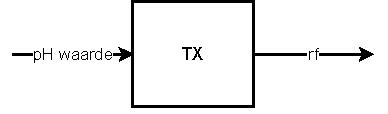
\includegraphics[width=0.9\textwidth]{rfBlock}
    \end{figure}

\end{frame}


\begin{frame}
    \frametitle{Ontvangstgevoeligheid}

    \begin{table}
        \centering
        \begin{tabular}{l|c}
            Eigenschap & Waarde \\\hline
            BER & $1\times10^{-5}$ \\
            $\Delta N$ & -105 dBm \\
            Noise Figure & 12.6 dB \\
            Modulatie & GFSK \\
        \end{tabular}
        \caption{Eigenschappen van de ontvanger op het basisstation.}
    \end{table}

    \pause 

    $S_{or}=-57$ dBm bij B = \qty{1}{\mega\hertz}

    $S_{or}=-54$ dBm bij B = \qty{2}{\mega\hertz}

\end{frame}

\begin{frame}
    \frametitle{Minimum zendvermogen}

    \begin{table}
        \centering
        \begin{tabular}{l|c}
            Eigenschap & Waarde \\\hline
            Afstand & \qty{10}{\meter} \\
            Hoogte & \qty{1}{\meter} \\
        \end{tabular}
        \caption{Antenne plaatsing.}
    \end{table}

    Path loss = 53.2 dB

    \pause

    $\Rightarrow$

    $P_{z}=-4$dBm bij B = \qty{1}{\mega\hertz}

    $P_{z}=-1$dBm bij B = \qty{2}{\mega\hertz}
\end{frame}

\begin{frame}
    \frametitle{Energie en gemiddeld vermogen}

    Energie kosten per verzonden pakket:
    \begin{equation*}
        E_{z,p}=\frac{l}{DR}P_z
    \end{equation*}

    \pause

    $E_{z,p}=$\qty{117.8}{\nano\joule} bij B = \qty{1}{\mega\hertz}

    $E_{z,p}=$\qty{117.6}{\nano\joule} bij B = \qty{2}{\mega\hertz}

    \pause

    \vspace{1cm}
    $\overline{P_z}=E_{z,p}f_s$ $\Rightarrow$ \qty{7.1}{\micro\watt} in geval van een bandbreedte van \qty{2}{\mega\hertz}

\end{frame}
\subsection{Batterij} \label{sec:battery}
In onderzoek \cite{BatteryComparison} is te zien dat Lithium-Polymeer batterijen (LiPo) een hoge energiedichtheid hebben in vergelijking met andere soorten batterijen. Er zijn anderen die hogere energie densiteit hebben, maar daarvan zijn de kosten hoog, of zijn er andere nadelige effecten\cite{BatteryComparison}. Dit heeft ervoor gezorgd dat voor de sensor module ontwerp een LiPo gekozen is als batterij. Spanning van een cel LiPo (1s) is maximaal 4.2 V en minimaal veilige spanning is 2.7 V\cite{BatteryComparison}.

\subsection{Energy Harvesting}

Vanuit de opdrachtdefinitie is er gekozen voor een piëzo element. Deze piëzo kan mechanische trillingen omzetten naar elekrsiche spanning. Deze spanning kan gebruikt worden om de accu op te laden of de vermogen gebruik van de module te verminderen. De peizo element kan beide indoor en outdoor gebruikt worden.


\subsection{Voeding} \label{sec:voeding} 

%!! TODO: energy harvesting, spanning, batterij laden, beveiliging, stroom. 

De voedingsspanning is gekozen vanuit de maximale spanning die nodig is voor de ISFET sensor\cite{isfet}. Hieruit volgt een maximale systeemspanning van 3.3 V. 


Zoals te lezen in \cref{sec:battery} is er gekozen voor LiPo batterij technologie. De batterij heeft een beveiliging voor beide op- en ontladen nodig. De celspanning moet omgezet worden naar systeemspanning van 3.3 V. Dit wordt op 2 manieren gedaan, met een DC-DC buck-boost converter en een low dropout regelaar(LDO). De buck-boost is efficiënter dan de LDO. Een voordeel van de LDO is dat de spanningsrimpel veel lager is dan bij een buck-boost. Daarom wordt de LDO gebruikt voor het voeden van de analoge uitleesschakeling. De buck-boost gaat naar het digitale deel. Als een microcontroller goed ontkoppeld is dan maakt het spanningsrimpel niet uit voor de werking van de microcontroller. Daardoor is de hogere rimpel spanning van de buck-boost niet een probleem voor de microcontroller. De voeding is schematisch te zien in \cref{fig:voedingSchematisch}.

Voor energy harvesting is er een piezo element gekozen. Een piezo element kan gezien worden als een AC bron. Deze AC bron moet omgezet worden naar DC die door het systeem gebruikt kan worden om de batterij mee op te laden. De AC bron wordt met een gelijkrichter naar DC omgezet. Deze DC spanning is niet hetzelfde als de systeemspanning dus die moet omgezet worden naar een spanning die de batterij in gaat, zodat de batterij kan opladen.

\begin{figure}[ht]
    \centering 
    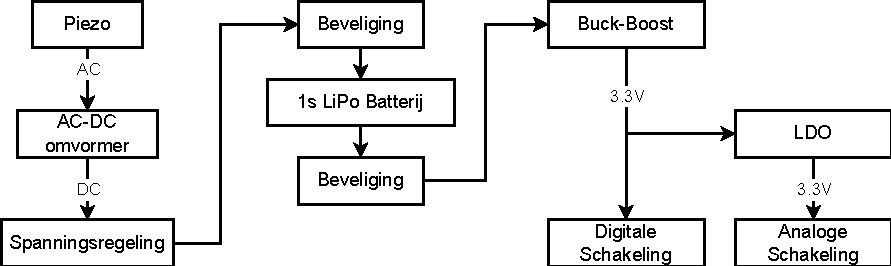
\includegraphics{voedingSchematisch.pdf}
    \caption{Voeding schematisch}
    \label{fig:voedingSchematisch}
\end{figure}



\subsection{Energie budget}
Voor het energiebudget zijn de waardes uit \cref{tab:energieBudgetEstimatie} gekozen. De waardes in \cref{tab:energieBudgetEstimatie} zijn boven de theoretisch berekend minium gebruik voor het systeem bepaald maar onder de 10 mW.


\begin{table}[ht]
    \centering
    \begin{tabular}{l|l}
        Func. blok          & Vermogen [mW] \\
        \hline                              
        Reken $U_{GS}\rightarrow$pH & 0.6   \\
        ADC                 & 1             \\
        AA-filter           & 0.2           \\
        Meet $U_{GS}$       & 0.2           \\
        Zenden              & 5             \\
        Oplader             & 0.5           \\
        Beveiliging         & 0.5           \\
        Spanningsregeling   & 1             \\ 
        \hline
        \hline
        Totaal              & 9
        
    \end{tabular}
    \caption{Energie budget}
    \label{tab:energieBudgetEstimatie}
\end{table}



\input{sections/energieBudget}






% \begin{table}[!htbp]
%     \centering
%     \begin{tabular}{|l|r|}
%         \hline
%         Ingangen    & Oplossing met een pH waarde tussen de 2 en 10 \\
%                     & Een temperatuur tussen de fliep en floep $^\circ$C \\
%         \hline
%         Uitgangen   & Een BLE RF signaal \\
%         \hline
%         Functie     & Meet de pH waarde van een oplossing en stuurt deze op naar een basisstation.  \\
%         \hline
%     \end{tabular}
%     \caption{Specificaties van }
%     \label{tab:in en uitgangen}
% \end{table}


% TODO: Moet gereformateerd zodat het past in dit formaat.
%% Haskell is mijn favoriete taal

Het signaalverwerkingsblok maakt een nuttig signaal van de te meten grootheid. Een uitbreiding van dit blok is te zien in \cref{fig:signaalverwerking}.
Van links naar rechts zijn de functies van de blokken als volgt:
\begin{enumerate}
    \item De grootheid, de pH-waarde, wordt gemeten. Dit wordt gedaan door de gate-source spanning $U_{GS}$ van de ISFET te meten.
    \item Het signaal wordt gefilterd om de bandbreedte te limiteren.
    \item Er wordt voor de kruisgevoeligheid van de pH-sensor gecompenseerd d.m.v. een temperatuursensor.
    \item De waarde van $U_{GS}$ wordt omgerekend naar de pH-waarde.
    \item Deze waarde wordt draadloos opgestuurd naar de ontvanger.
\end{enumerate}
Het `enable' blok wordt gebruikt om het signaalverwerkingsonderdeel van het systeem te activeren en te deactiveren. Op deze manier hoeft het systeem alleen maar aan te staan wanneer het nodig is, en wordt er minder energie verbruikt.

% \begin{figure}[!htb]
%     \centering
%     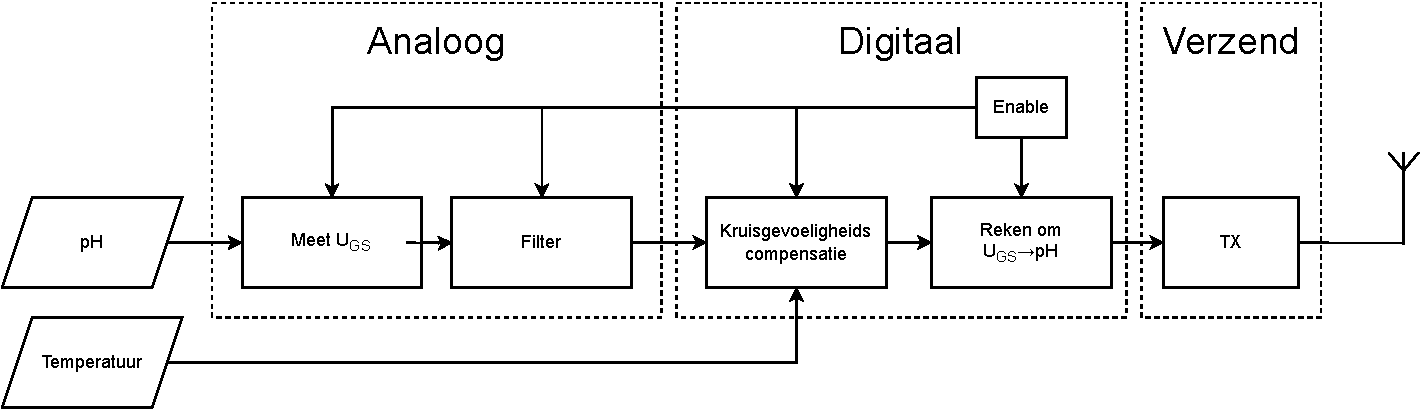
\includegraphics[width=\textwidth]{meetGedeelte.pdf}
%     \caption{Het signaalverwerkende onderdeel van het systeem, onderverdeeld naar het analoge en digitale domein.}
%     \label{fig:signaalverwerking}
% \end{figure}



\begin{figure}[!htb]
    \centering
    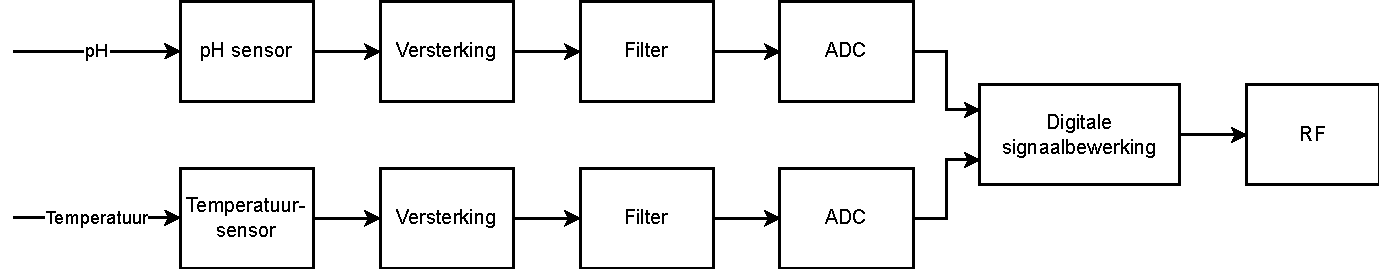
\includegraphics[width=0.95\textwidth]{analogeBewerkingsFunctie}
    \caption{Het analoge gedeelte van de signaalbewerking.}
    \label{fig:analogeBewerkingsFunctie}
\end{figure}


\begin{figure}[!htb]
    \centering
    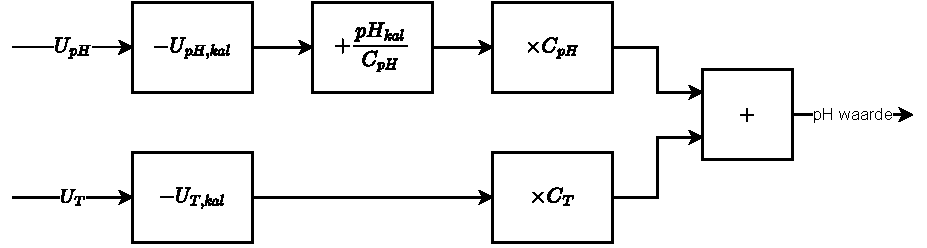
\includegraphics[width=0.95\textwidth]{digitaleBewerkingsFunctie}
    \caption{Het digitale gedeelte van de signaalbewerking.}
    \label{fig:digitaleBewerkingsFunctie}
\end{figure}



% TODO: TAAL
\subsection{Spanningsregeling}
Voor spanningsregeling zijn er meerdere componenten nodig, zoals te zien in \cref{fig:spanningsregeling}. De energy harvesting produceert een spanning, die omgezet moet worden naar iets de rest van het systeem iets mee kan. Deze omgevormde spanning kan dan zowel gebruikt worden voor het opladen van de batterij, als het voeden van de rest van het systeem.
Om de batterij op te laden is een batterijregelingssysteem (BMS) nodig. De BMS kan via een beveiliging de batterij opladen. De beveiliging limiteert de batterijspanning en -stroom. De tweede beveiliging zit tussen de batterij en de rest van het systeem. Deze beveiliging zorgt ervoor dat er niet te veel stroom uit de batterij getrokken wordt, waardoor deze kapot kan gaan. De spanningsregelaar zet de spanning die uit de batterij komt om naar een spanning die gebruikt kan worden door de rest van het systeem.

\begin{figure}[!htb]
    \centering
    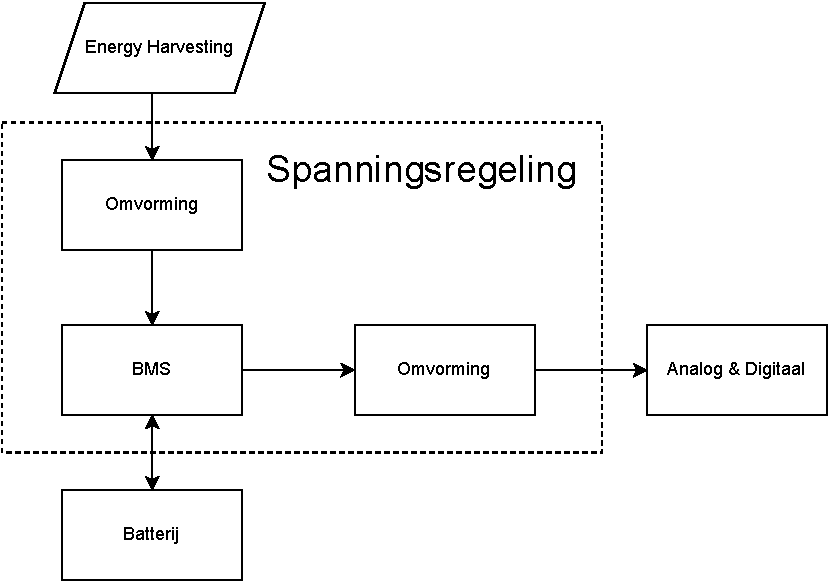
\includegraphics[width=0.7\textwidth]{spanningsRegeling3.drawio.pdf}
    \caption{Het Spanningsregeling van het systeem.}
    \label{fig:spanningsregeling}
\end{figure}

\subsection{RF}
In \cref{fig:functional} is het TX blok het blok dat de data draadloos verstuurt. Dit blok zal direct ingekocht worden; er zijn meer dan genoeg kant-en-klare oplossingen beschikbaar om de functie van dit blok te vervullen.


\subsection{Microcontroller}
Een gedeelte van de signaalverwerking zal gebeuren in het digitale domein. Hiervoor is een microcontroller de voor de hand liggende oplossing. Bij het kiezen van een microcontroller moet er een aantal eigenschappen overwogen worden. Een paar van deze eigenschappen zijn:
\begin{itemize}
    \item gebruikte vermogen,
    \item mogelijke slaapstanden,
    \item beschikbare peripherals,
    \item kloksnelheid,
    \item geheugen,
    \item programmeergeheugen
    \item en de prijs.
\end{itemize}



    \newpage

    \section{Realisatie}
In \cref{sec:ontwerp} is voor elk onderdeel van het systeem besproken wat de eisen zijn van dat onderdeel. Dit hoofdstuk gaat in op de implementatie van elk van deze systeemonderdelen.

\subsection{Spanningsreferentie}
Zoals besproken in \cref{sec:referenceVoltage} kunnen de weerstandswaardes van de spanningsreferentie erg hoog gekozen worden. Met een $R_1$ van \qty{5.6}{\mega\ohm} gebruikt de spanningsdeler \qty{1.65}{\micro\watt}.

Volgens \cref{eq:dividerNoise} heeft de condensatorwaarde wel effect op de ruis. Met een condensator van \qty{1}{\micro\farad} produceert de spanningsreferentie \qty{64.4}{\nano\volt} aan ruis. Dit zorgt voor een signaal-ruis verhouding van \qty{138}{\decibel}, wat meer dan genoeg is.

Deze gekozen waardes en de resulterende eigenschappen zijn te vinden in \cref{tab:divider}.

\begin{table}[!htbp]
\centering
\begin{tabular}{l|l|l}
    Symbool & Waarde & Eenheid \\
    \hline
    $R_1$       & 5.6  & $\si{\mega\ohm}$   \\
    $R_2$       & 1.0  & $\si{\mega\ohm}$   \\
    $C$         & 1.0  & $\si{\micro\farad}$\\
    $P$         & 1.65 & $\si{\micro\watt}$ \\
    $u_{n,out}$ & 64.4 & $\si{\nano\volt}$  \\
    SNR         & 138  & $\si{\decibel}$
\end{tabular}
\caption{De gekozen waardes van de spanningsdeler, met het resulterende vermogensverbruik en de ruiseigenschappen.}
\label{tab:divider}
\end{table}


\subsection{Microcontroller}
Het digitale gedeelte van het energieverbruik kan opgedeeld worden in 3 onderdelen: de ADC, de digitale signaalverwerking (\cref{fig:digitaleBewerkingsFunctie}) en het draadloos versturen van data. Het is mogelijk om elk van deze onderdelen met aparte componenten te implementeren. Er zijn echter ook componenten beschikbaar die al over elk van deze functionaliteiten beschikken.

Een voorbeeld van een dergelijk component is de nRF52810. Deze microcontroller beschikt over meerdere 14 bit ADC kanalen\footnote{De ADC kanalen zijn alleen 14 bit met oversampling.} en een ingebouwde 2.4GHz Bluetooth transceiver.
Ook heeft de microcontroller een slaapstand die onderbroken kan worden door een ingebouwde RTC, wat nuttig is voor het periodiek samplen en versturen van pH waardes. In deze slaapstand wordt er zo'n \qty{1.5}{\micro\ampere} gebruikt. Met een voedingsspanning van \qty{3.3}{\volt} komt dit uit op een vermogensverbruik van \qty{4.95}{\micro\watt}. Daarbij heeft de microcontroller ook de mogelijkheid om onderdelen van het geheugen uit te zetten, wat tot meer energiebesparing kan leiden \cite{nrf52810}.


\subsection{ADC}
De specificaties van de ADC die nodig is voor dit project kunnen berekend worden op basis van de specificaties voor het ADC blok. Deze specificaties staan in \cref{tab:systemSpecADC} samengevat.
\begin{table}[!htbp]
    \centering
    \begin{tabular}{l|c|l}
        Symbol      & Waarde & Eenheid\\\hline
        $SNR_{in}$  & 37        & dB\\
        NF          & 3         & dB\\
        $u_{in}$    & 2.5       & mV\\
    \end{tabular}
    \caption{De eisen voor het omzetten van het analoge signaal naar een digitaal signaal.}
    \label{tab:systemSpecADC}
\end{table}

Door gebruik te maken van de formules uit \cref{sec:ADC:numBits,sec:ADC:sampleFreq} kunnen de specificaties voor de benodigde ADC berekend worden. De resultaten hiervan zijn in  \cref{tab:specADC} geplaatst.

Bij het berekenen van deze specificaties is er van uit gegaan dat het totale noise figure 1 op 1 is verdeeld tussen de resolutie en de bemonsteringsfrequentie.
\begin{table}[!htbp]
    \centering
    \begin{tabular}{l|c|l}
        Symbol      & Waarde    & Eenheid\\\hline
        n           & 14        & bits\\
        $f_{s,min}$ & 45        & Hz\\
        $f_{s,max}$ & 515       & kHz\\
    \end{tabular}
    \caption{De eisen voor het omzetten van het analoge signaal naar een digitaal signaal.}
    \label{tab:specADC}
\end{table}

Het blijkt het geval te zijn dat de ingebouwde ADC die in de \mcu  zit, voldoet aan de specificaties die in \cref{tab:specADC,tab:systemSpecADC} staan \cite{nrf52810}. Dit zorgt er voor dat het niet nodig is om een externe ADC te gebruiken.

\subsection{Filter}
Het laagdoorlaatfilter dat voor de ADC zit, heeft een weerstand en een condensator die van een waarde voorzien moeten worden.
Met de ruis van het voorgaande systeem kan de minimale condensatorwaarde berekend worden door middel van \cref{eq:filterCapMin}. Deze komt uit op ongeveer \qty{60}{\pico\farad}. Hiermee moet de weerstandswaarde echter \qty{270}{\mega\ohm} zijn, wat niet praktisch is. Met een condensator van \qty{10}{\nano\farad} kunnen de waardes in \cref{tab:filterValues} berekend worden. Deze waardes vallen binnen de specificaties.

\begin{table}[!htbp]
    \centering
    \begin{tabular}{l|l|l}
        Symbool & Waarde & Eenheid \\
        \hline
        $C$         & 82    & $\si{\nano\farad}$\\
        $R$         & 180   & $\si{\kilo\ohm}$  \\
        $f_c$       & 10.8  & $\si{\hertz}$     \\
        $P$         & 408   & $\si{\nano\watt}$ \\
        $u_{n,out}$ & 225   & $\si{\nano\volt}$ \\
        NF          & 0.23  & $\si{\decibel}$   \\
    \end{tabular}
    \caption{De gekozen waardes van het filter, en de resulterende vermogens- en ruiseigenschappen.}
    \label{tab:filterValues}
\end{table}

Nu de waardes van het filter bekend zijn moet gecontroleerd worden of de ADC nog steeds aan de specificaties voldoet. Het is nodig om dit te controleren omdat het filter passief is geïmplementeerd. Door de passieve implementatie ontstaat er een spanningsdeler. Deze spanningsdeler wordt gevormd door de ingangsimpedantie van de ADC en de weerstandswaarde van het anti-aliasing filter. Uit \cref{eq:calcMinNumberADCbits} blijkt echter dat de eisen voor de ADC niet veranderen en dat de interne ADC van de \mcu nog steeds gebruikt kan worden.


\subsection{Nullor implementatie}
Voor de nullor die gebruikt wordt om de ISFET uit te lezen in \cref{sec:ISFETLees} moet een implementatie gekozen worden. De uitleesschakeling mag volgens de specificaties maximaal \qty{200}{\micro\watt}  gebruiken. De constante stroom die door de weerstand en ISFET in \cref{fig:measureResistor} heen loopt, zorgt voor een constant vermogensverbruik van \qty{165}{\micro\watt}. Hierdoor mag de nullor implementatie maximaal \qty{35}{\micro\watt} gebruiken. Het maximale dynamische vermogen dat deze nullor implementatie aan de uitgang zal moeten kunnen leveren, is gelijk aan het maximale vermogen dat het filter kan dissiperen. Er blijft dan afgerond nog \qty{34}{\micro\watt} aan statisch vermogen over. Dit resulteert in een maximale quiescent stroom van \qty{10.3}{\micro\ampere}.

De uitleesschakeling moet een minimale SNR hebben van 40 dB. De maximale ruisspanning en stroom die de nullor mag genereren aan de ingang zijn te berekenen met \cref{eq:nullorImplementNoise}. Deze vergelijking is afgeleid uit \Cref{eq:measureNoiseFull}.
\begin{equation} \label{eq:nullorImplementNoise}
    S_{u_{{n,n}}} + S_{i_{{n,in}}}\left(Z_{fet} // R\right)^2 = \frac{S_{u_{{n,out}}}}{H^2(\ph)} - S_{u_{{n,ref}}}
\end{equation}

De LTC2064 opamp heeft (buiten shutdown) een quiescent stroom van \qty{2.5}{\micro\ampere}, wat op \qty{3.3}{\volt} resulteert in een vermogen van \qty{8.25}{\micro\watt}. Daarbij heeft deze een spectrale ruisdichtheid van \qty{12}{\femto\ampere\hertz^{-0.5}} en $\qty{220}{\nano\volt\hertz^{-0.5}}$\cite{LTC2064}. Dit zit volgens \cref{eq:nullorImplementNoise} ver onder het maximum. Daarnaast is zowel de ingangsafwijking als de 1/f ruis van deze opamp erg laag. Hierdoor is deze opamp gekozen voor het ontwerp.

\subsection{Rf}
In \cref{sec:ontwerp:Rf} is ingegaan op het minimum zendvermogen dat nodig is. Dit minimum vermogen is \qty{7.1}{\micro\watt}. Het is belangrijk om op te merken dat dit enkel het minimum vermogen is dat in het rf signaal zit. Het genereren van dit rf signaal kan mogelijk meer energie kosten. Bij het kiezen van de microcontroller is de \mcu gekozen, onder andere omdat er een \qty{2.4}{\giga\hertz} transceiver in zit. Uit de datasheet van de \mcu is te halen dat deze transceiver \qty{4.6}{\milli\ampere} aan stroom trekt, indien er draadloos wordt gezonden met \qty{0}{\deci\belmilliwatt} en een datasnelheid van \qty{1}{\mega\hertz} \cite{nrf52810}. Door \cref{eq:calcPperPacket,eq:calcRfAvaragePower} te gebruiken is een gemiddeld rf vermogen van \qty{45}{\micro\watt} te berekenen. \qty{45}{\micro\watt} zit onder het energie budget dat beschikbaar is voor het draadloos zenden.

Bij de implementatie van het rf zenden, is het belangrijk om de rf uitgangsimpedantie van de \mcu te matchen met de antenne impedantie. Dit is belangrijk om een zo klein mogelijke hoeveelheid aan energie te verspillen aan reflecties \cite{FundamentalsofAppliedElectromagnetics}. In de datasheet van de \mcu staat al beschreven hoe de rf uitgang gematcht kan worden aan \qty{50}{\ohm} \cite{nrf52810}. Deze impedantie matching wordt gedaan op basis van een L-type matching netwerk. Hierbij staat er een spoel in serie met de antenne en een condensator parallel aan de rf uitgang van de \mcu \cite{nrf52810}.
\subsection{Batterij en bescherming}

Voor de gekozen LiPO batterij technologie is er bescherming nodig. De celspanning mag niet boven de 4.2 V of onder de 2.7 V komen. Dit kan op meerdere manieren gedaan worden. In de implementatie van de sensor module is er gekozen voor een LTC4071 batterij beschermings IC. Wanneer de spanning van de batterij boven de 4.2 V komt, gebruikt de LTC4071 een 50mA shunt om de ingang stroom naar hitte om te zetten. Wanneer de batterijspanning onder de 2.7 V komt, zet de IC de uitgang uit, om te voorkomen dat de batterijspanning verder daalt.

\subsection{Voeding}
Voor de voeding is er gekozen voor een LTC3330 van Analog Devices. Dit is een zogenaamde `power management integrated circuit' (PMIC). Deze PMIC voldoet aan de specs van \cref{tab:systemSpecs}, en heeft een aantal nuttige eigenschappen:
\begin{itemize}
    \item Ingebouwde ideale diodes voor AC-DC omzetting
    \item Een buck-boost converter
    \item Een low dropout regulator (LDO)
    \item Mogelijkheid om de LDO uit te zetten
    \item Lage 750 nA quiescent current
\end{itemize}

De gekozen PMIC is een IC die is ontworpen voor energy harvesting en low power modules. De uitgang van de energy harvesting wordt als eerste gelijkgericht door een ideale diode gelijkrichter. Dit zorgt voor minimaal energie verlies. Hierna bepaalt de LTC3330 of de rest van het systeem de stroom nodig heeft of dat de energie opgeslagen moet worden in de accu. De PMIC heeft 2 spanning omzet methodes ingebouwd. Een buck-boost converter en een LDO die aan en uit kan. De LDO wordt gevoed door de buck-boost.

\begin{figure}
    \centering

    \label{}
\end{figure}

% software
% hardware

\subsection{Printplaten}
De schakelingen voor de voeding en voor het uitlezen van de ISFET zijn opgedeeld in twee verschillende printplaten. Dit is gedaan zodat beide schakelingen apart van elkaar getest kunnen worden. De uitlees PCB is te zien in \cref{fig:sensorPCB}. Deze PCB bevat de ISFET uitleesschakeling en de \mcu, die de gemeten pH waarde naar het basisstation opstuurt. De voeding printplaat is te zien in \cref{fig:powerPCB}. Deze PCB regelt de energy harvesting, samen met het veilig opladen en het ontladen van de batterij. De twee printplaten zijn met elkaar verbonden door middel van pin headers. Beide schakelingen zijn te zien \cref{fig:PCBs}.

Beide PCB's hebben op elk belangrijk signaal een testpunt. Op deze manier kan er eenvoudig gemeten worden.


\begin{figure}[!htbp]
    \centering
    \begin{subfigure}[b]{0.48\textwidth}
        \centering
        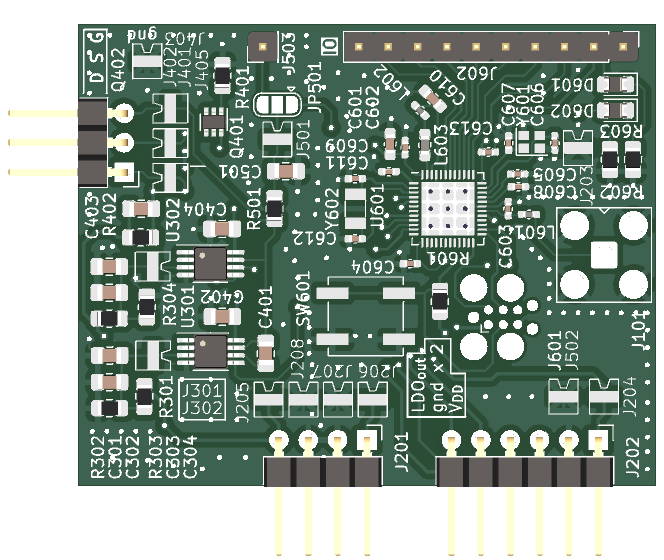
\includegraphics[width=\textwidth]{sensorBord}
        \caption{De ISFET uitlezende PCB.}
        \label{fig:sensorPCB}
    \end{subfigure}
    \hfill
    \begin{subfigure}[b]{0.60\textwidth}
        \centering
        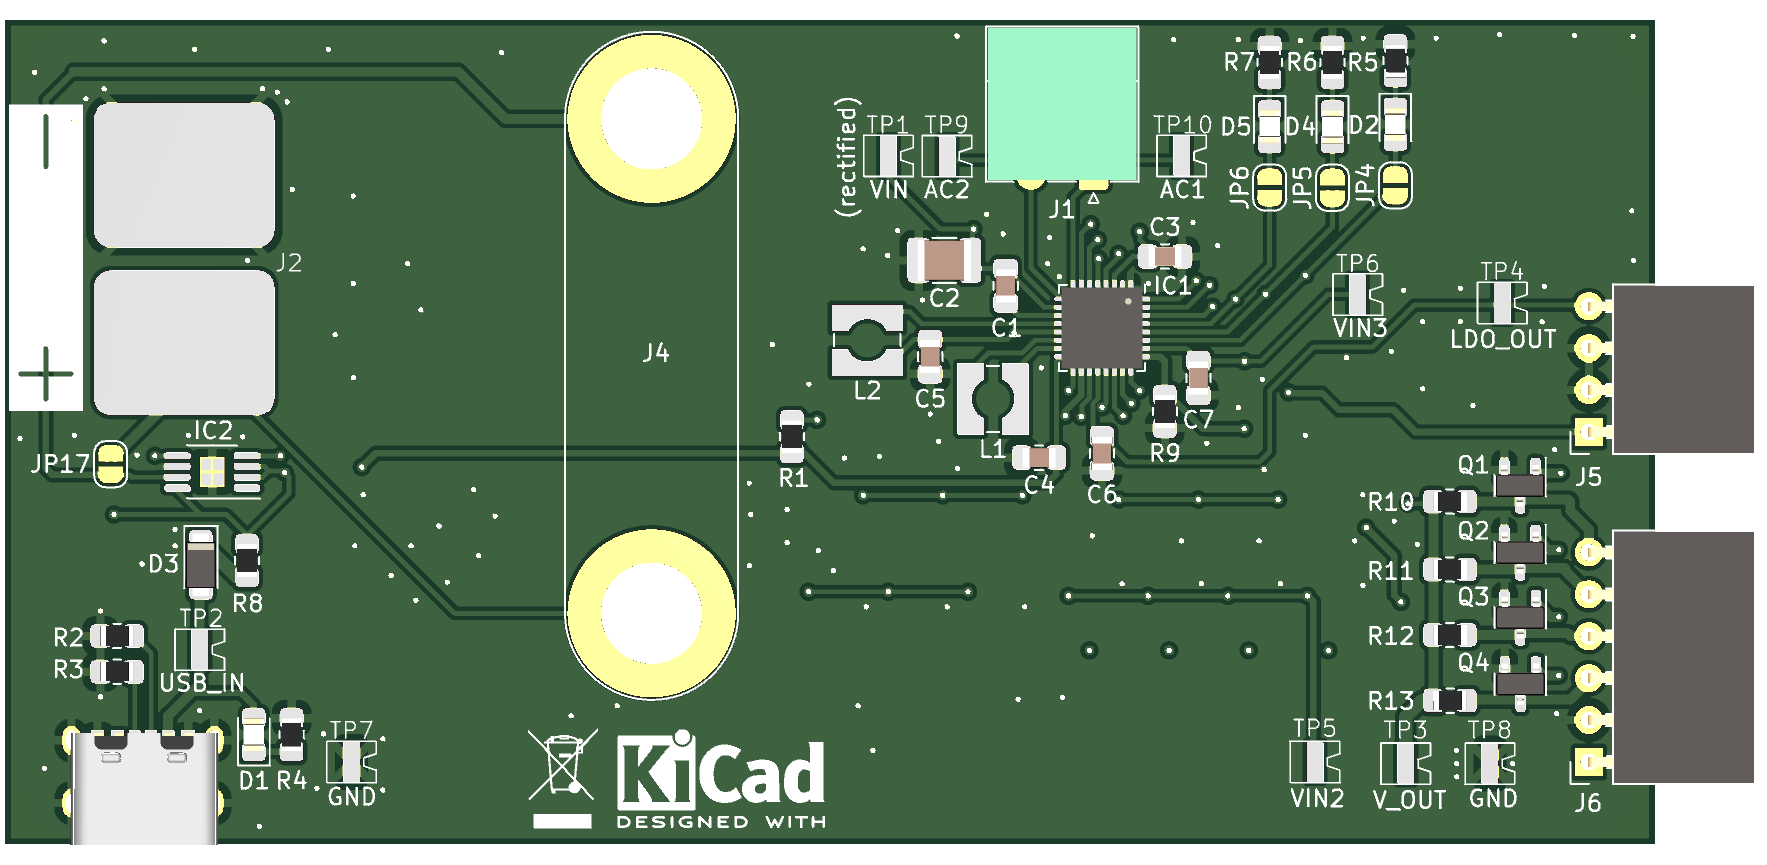
\includegraphics[width=\textwidth]{powerandharvest}
        \caption{De voeding en harvesting PCB.}
        \label{fig:powerPCB}
    \end{subfigure}
    \caption{De gemaakte PCB's.}
    \label{fig:PCBs}
\end{figure}

    \newpage

    \section{Bepalen testplan(nen)}


    \newpage

    % \section{Uitvoering Testplan(nen) en bespreking testresultaten}

    % \newpage

    \section{Discussie}

% analyse van project 

% opmerkingen over verloop project

% opmerkingen over systeem


    \newpage

    \section{Conclusie}

    \newpage

    \section{Aanbevelingen}


    \newpage

    \printbibliography[heading=bibintoc]


    \newpage

    % \newpage

    \newpage
    \appendix
    \newpage
    \documentclass[12pt, a4paper, twoside]{article}

\usepackage[dutch]{babel}
\usepackage{hvaTemplate}
\usepackage{csquotes}
\usepackage[backend=biber, style=ieee]{biblatex}
\usepackage{siunitx}
\usepackage{pgfplots}

\addbibresource{references.bib}

% \setAuthor{\\\underline{Tycho Jöbsis (500845792)}\\ Jochem Leijenhorst (500855372)\\ Illya Ustenko (500845492)\\ Groep 7}
\setAuthor{
    \\Groep 7
    \begin{table}[h!]
        \centering
        \begin{tabular}{ll}
            \underline{Tycho Jöbsis} & (500845792)\\ 
            Jochem Leijenhorst       & (500855372)\\ 
            Illya Ustenko            & (500845492)        
        \end{tabular}
    \end{table}
}
\extraInfo{Sensor modules\\Datum metingen: 27 November 2023}
\setTitle{De fittingscoefficient voor pathloss meten}

\graphicspath{ {img/} }

\numberwithin{equation}{section}

% \begin{table}[h!]
%     \centering
%     \begin{tabular}{l|l}
%         \underline{Tycho Jöbsis} & (500845792)\\ 
%         Jochem Leijenhorst       & (500855372)\\ 
%         Illya Ustenko            & (500845492)        
%     \end{tabular}
% \end{table}

\begin{document}
    \makeTitlepage
    \authorsCopyright
    \onecolumn
    \subsection{Samenvatting}
Om een inschatting te kunnen maken wat het minimale zendvermogen moet zijn voor een bepaalde draadloze applicatie moet er een inschatting worden gemaakt hoeveel signaalverlies er optreed (path loss). In dit meetrapport worden een aantal modellen getoond die hierbij helpen. Een van deze modellen bevat een fittingscoëfficiënt. Door middel van het doen van metingen is er een waarde voor deze fittingscoëfficiënt gevonden.
% intro
% meeting
% conclusie
\subsection{Abstract}
To estimate the minimum transmission power required for a specific wireless application, it is necessary to assess the anticipated signal loss (path loss). This measurement report presents several models that assist in the estimation of path loss. One of these models includes a fitting coefficient. Through conducted measurements, a value for this fitting coefficient has been determined
    \newpage
    \tableofcontents

    \newpage
    \section{Introduction}
    \newpage
    \section{Meetopstelling}
In \autoref{sec:introduction} is een model beschreven waarmee path loss kan worden gemodelleerd. In dat model wordt er gebruik gemaakt van een fittingscoëfficiënt. Deze fittingscoëfficiënt kan echter anders zijn afhankelijk van de omgeving. Om een indicatie te krijgen van welke waarde de fittingscoëfficiënt heeft in het Jacoba Mulder Huis zal in dit hoofdstuk een testopstelling worden toegelicht waarmee geprobeerd wordt om de fittingscoëfficiënt te bepalen.

% \subsection{Meetopstelling}
Voor de metingen is gebruik gemaakt van de materialen die in \autoref{tab:measurement:materials} staan. Deze materialen zijn volgens ... opgesteld. Hierbij staan beide antennes op 1 meter hoogte en in eerste instantie op 1 meter afstand. Vervolgens is er met de signaal generator vanaf -10dBm in stappen van 2dBm tot 4dBm gezonden. Per zendniveau is er vervolgens met de R\&S spectrumanalyzer gemeten wat het ontvangst vermogen is. Nadat voor al de verschillende zendvermogens het ontvangst vermogen is gemeten wordt de afstand tussen de antennes vergroot met een meter.
\begin{table}[ht]
    \centering
    \begin{tabular}{l|l|l}
        Apparaat                            & Serienummer   & Beschrijving \\\hline
        Rigol                               & ...           & Signaalgenerator \\
        Rhode\&Schwarz FSP                  & ...           & Spectrumanalyzer \\
        BNC kabel                           & n.v.t         & BNC kabel van 1 meter \\
        BNC kabel                           & n.v.t         & BNC kabel van 1 meter \\
        BNC $->$ sma adapter                & n.v.t         & BNC male naar SMA female adapter \\
        BNC $->$ N-type adapter             & n.v.t         & BNC male naar N-type female adapter \\
        2.45GHz antenne ($G_{t/r}=2.5$dBi)  & n.v.t         & 2.45GHz antenne (YGL001AA) \\
        2.45GHz antenne ($G_{t/r}=2.5$dBi)  & n.v.t         & 2.45GHz antenne (YGL001AA) \\\hline
    \end{tabular}
    \caption{Materialen die zijn gebruikt voor de metingen in dit meetrapport}
    \label{tab:measurement:materials}
\end{table}
% place figure of measurement schematic


% Description of measurement setup

% Location of measurements

% Table of serial numbers of the used equipement
    \newpage
    \section{Resultaten}
In \cref{fig:pathLossMesurment} is te zien wat de gemeten waardes zijn van de testopstelling die is beschreven in \cref{sec:methods}. Hierbij is de horizontale as de afstand tussen de twee antennes, en is de verticale as het vermogen van de ontvangen signalen. 
\begin{figure}[ht]
    \centering
\begin{tikzpicture}
    \begin{axis}[
        title={},
        xlabel={Afstand (m)},
        ylabel={RSS (dBm)},
        grid=major,
        cycle list name=color list,
        no markers,
        every axis plot/.append style={thick},
        legend pos=outer north east,
        legend style={font=\small}
    ]
    \addlegendimage{empty legend}
    \addplot table [x=Distance,y=-10] {sections/data.dat};
    \addplot table [x=Distance,y=-8] {sections/data.dat};
    \addplot table [x=Distance,y=-6] {sections/data.dat};
    \addplot table [x=Distance,y=-4] {sections/data.dat};
    \addplot table [x=Distance,y=-2] {sections/data.dat};
    \addplot table [x=Distance,y=0] {sections/data.dat};
    \addplot table [x=Distance,y=2] {sections/data.dat};
    \addplot table [x=Distance,y=4] {sections/data.dat};
    \addplot table [x=Distance,y=6] {sections/data.dat};
    \addlegendentry{\hspace{-.6cm}\textbf{TSS}}
    \addlegendentry{-10 dBm}
    \addlegendentry{-8 dBm}
    \addlegendentry{-6 dBm}
    \addlegendentry{-4 dBm}
    \addlegendentry{-2 dBm}
    \addlegendentry{-0 dBm}
    \addlegendentry{-8 dBm}
    \addlegendentry{2 dBm}
    \addlegendentry{4 dBm}
    \addlegendentry{6 dBm}
    \end{axis}
\end{tikzpicture}

%TODO: Add better title?
\caption{RSS (Received Signal Strength) over afstand.}
\label{fig:pathLossMesurment}

\end{figure}

Bij deze meting was het meten van het ontvangst vermogen niet het doel. Het doel van de meting was namelijk het meten van het signaalverlies tussen een zend en ontvangstantenne. Door het ontvangen signaalvermogen min het zendvermogen te berekenen is het signaalverlies te bepalen. Dit wordt getoond in \cref{fig:pathLossMesurment:pathloss}. 
\begin{figure}[ht]
    \centering
\begin{tikzpicture}
    \begin{axis}[
        title={},
        xlabel={Afstand (m)},
        ylabel={PL (dB)},
        grid=major,
        cycle list name=color list,
        no markers,
        every axis plot/.append style={thick},
        legend pos=outer north east,
        legend style={font=\small}
    ]
    \addlegendimage{empty legend}
    \addplot table [x=Distance,y=-10] {sections/data2.dat};
    \addplot table [x=Distance,y=-8] {sections/data2.dat};
    \addplot table [x=Distance,y=-6] {sections/data2.dat};
    \addplot table [x=Distance,y=-4] {sections/data2.dat};
    \addplot table [x=Distance,y=-2] {sections/data2.dat};
    \addplot table [x=Distance,y=0] {sections/data2.dat};
    \addplot table [x=Distance,y=2] {sections/data2.dat};
    \addplot table [x=Distance,y=4] {sections/data2.dat};
    \addplot table [x=Distance,y=6] {sections/data2.dat};
    \addlegendentry{\hspace{-.6cm}\textbf{TSS}}
    \addlegendentry{-10 dBm}
    \addlegendentry{-8 dBm}
    \addlegendentry{-6 dBm}
    \addlegendentry{-4 dBm}
    \addlegendentry{-2 dBm}
    \addlegendentry{-0 dBm}
    \addlegendentry{-8 dBm}
    \addlegendentry{2 dBm}
    \addlegendentry{4 dBm}
    \addlegendentry{6 dBm}
    \end{axis}
\end{tikzpicture}

%TODO: Add better title?
\caption{Signaalverlies over afstand.}
\label{fig:pathLossMesurment:pathloss}

\end{figure}



    \newpage
    \section{Discussion}
    \newpage
    \subsection{Conclusie}
In dit meetrapport is er gemeten wat de fittingscoëfficiënt voor de path loss in het Jacoba Mulder Huis is. In de analyse van de gemeten data is naar voren gekomen dat de gemeten data niet betrouwbaar genoeg is om een eenduidige waarde te vinden voor de fittingscoëfficiënt. Aangezien een hogere fittingscoëfficiënt meer energie kost maar er wel voor zorgt dat een systeem het minimale bereik kan halen, wordt er aangeraden om voorlopig voor de fittingscoëfficiënt $l_f$ een waarde van 7.80 te gebruiken. 
% Make a conclusion. Broader then the discussion.

    % \newpage
    \printbibliography

    \newpage
    \appendix

\end{document}


    
\end{document}

